% !TEX program = xelatex
\documentclass[11pt,a4paper]{article}

\usepackage[margin=24mm]{geometry}
\usepackage{fontspec}
\usepackage{booktabs}
\usepackage{array}
\usepackage{graphicx}
\usepackage{xcolor}
\usepackage{tikz}
\usepackage{microtype}
\usepackage{setspace}
\usepackage{caption}
\usepackage{hyperref}
\usepackage{enumitem}
\usepackage{amsmath,amssymb}
\usepackage{fancyhdr}
\usepackage{titlesec}
\usepackage{xspace}

\newcommand{\app}{\textsf{APP}\xspace}

\setmainfont{DejaVu Serif}
\setmonofont{DejaVu Sans Mono}

\usetikzlibrary{arrows.meta,positioning}

\definecolor{Rec}{HTML}{888888}
\definecolor{APC}{HTML}{0077BB}
\definecolor{APCp}{HTML}{88CCEE}
\definecolor{FS}{HTML}{EE7733}
\definecolor{FSp}{HTML}{F4A582}
\definecolor{Ink}{HTML}{1A1A1A}
\definecolor{Mute}{HTML}{5C5C5C}
\definecolor{Paper}{HTML}{F7F5F1}
\definecolor{Rule}{HTML}{D9D4CC}

\pagecolor{Paper}
\color{Ink}
\hypersetup{
  colorlinks=true,
  linkcolor=Ink,
  citecolor=Ink,
  urlcolor=APC,
  pdftitle={ForkServe: Branch-Aware Prefill Pruning for Efficient vLLM Serving},
}

\pagestyle{fancy}
\fancyhf{}
\setlength{\headheight}{22pt}
\fancyhead[L]{\small\color{Mute}Branch-aware prefill pruning on vLLM}
\fancyhead[R]{\small\color{Mute}Qwen3-14B / Qwen3-8B / DeepSeek-R1 8B}
\fancyfoot[C]{\small\color{Mute}\thepage}
\renewcommand{\headrulewidth}{0.3pt}
\renewcommand{\headrule}{\hbox to\headwidth{\color{Rule}\leaders\hrule height \headrulewidth\hfill}}

\titleformat{\section}{\large\bfseries}{\thesection}{0.8em}{}
\titleformat{\subsection}{\normalsize\bfseries}{\thesubsection}{0.8em}{}
\captionsetup{font=small,labelfont={bf,color=Mute},textfont={color=Mute}}
\setlist[itemize]{leftmargin=1.4em,itemsep=0.25em}
\setstretch{1.15}

\title{\textbf{ForkServe: Branch-Aware Prefill Pruning}\\[0.35em]
{\large Efficient vLLM serving of Tree-of-Thoughts and ReAct}}
\author{%
\begin{tabular}[t]{c}
Dong Liu \hspace{1.4em} Hao Wu \hspace{1.4em} Chuan Wu \\[0.55em]
The University of Hong Kong
\end{tabular}%
}
\date{}

\begin{document}
\maketitle
\vspace{-1.6em}

\begin{abstract}
\noindent
We treat ForkServe as \emph{efficient vLLM serving} of branched Tree-of-Thoughts and ReAct.
The serving object is the branch, not the request.
\texttt{fork} is a pointer swap: trunk pages stay read-only, the child's page table aliases them ($\mathrm{refcount}{=}k$), and no KV is memcpy'd.
That already matches APC's prefill work $W{=}L{+}k\bar\ell$ without cloning the trunk.
The remaining expand cost is residual prefill that APC and stock disaggregated prefill still pay for every sibling.

Advanced prefill pruning (\app) sits between those two mechanisms and decides, per residual, whether a GPU kernel---and later a connector \texttt{insert}---should run at all.
Four skip layers run cheapest first: a hash index skips published full blocks; a draft score drops illegal or looping siblings before they start; an early-prefix check cancels in-flight chunks; the disaggregated gate inserts only survivors.
The winner index is always retained, so the committed token sequence is unchanged.
Decoding acceleration then stops winner generation at an answer marker (\texttt{\#\#\#\#}, \texttt{\textbackslash boxed}, \texttt{</think>}) instead of padding to $D$, and keeps committed decode ahead of speculative prefill in a two-class scheduler.

Baselines are \emph{recompute} (prefix cache off) and \emph{APC} (automatic prefix caching).

On Qwen3-14B GSM8K ($n{=}1319$, $\mathrm{tp}{=}2$) peak resident KV is below APC on every batch (median $1030$ vs.\ $1430$, ratio $0.72$), accuracy is $0.845$ vs.\ $0.844$, and generation is $18.9$ vs.\ $18.6$ minutes.
The same KV ordering holds on Qwen3-8B, Qwen3-14B, and DeepSeek-R1-Distill-Llama-8B math suites at $\mathrm{tp}{=}2$ and $\mathrm{tp}{=}4$ ($0.58$--$0.80\times$ APC).
An analytical concurrency sweep from measured DeepSeek GSM8K peaks raises SLO-feasible QPS from $192$ to $256$ ($+35\%$ saturated decode tok/s).

Control-plane APP (setting L) is the only method that both aliases the trunk and drops low-score residuals: modeled fan-out $35.9$\,ms vs.\ $139$\,ms for APC, peak KV $2880$ vs.\ $11520$.
A GPU run of the same stack on Qwen3-8B (setting M: $80$ items, $D{=}512$) confirms the KV gap and the decode-stop gain.
On GSM8K, ForkServe+ emits $13356$ decode tokens vs.\ $40960$ for APC at $\mathrm{tp}{=}2$ ($0.33\times$) and finishes in $28.2$\,s vs.\ $36.0$\,s; at $\mathrm{tp}{=}4$ it is $12826$ vs.\ $40960$ tokens and $16.9$\,s vs.\ $22.7$\,s, with accuracy $0.925$ vs.\ $0.938$.
Peak KV stays $1182$ vs.\ $1582$ ($0.75\times$ APC) at both widths.
Setting N repeats the same four-system forest on six models ($n{=}40$): GSM8K peak KV is $0.72$--$0.75\times$ APC on every family, and Game24 is $0.57$--$0.62\times$; answer-marker stop remains model-dependent.
\end{abstract}

\section{Design}
\label{sec:design}

vLLM already has two ways to avoid recomputing a shared trunk: automatic prefix caching reuses a block after it is published, and disaggregated prefill moves whatever KV the prefiller computed.
Neither decides \emph{which} residuals of a Tree-of-Thoughts or ReAct fan-out are worth a GPU kernel.
ForkServe makes that decision a serving primitive.

\paragraph{Pointer-swap fork.}
\texttt{open} materializes the trunk $L$ once as read-only copy-on-write pages.
\texttt{fork} installs $k$ child page tables that alias those pages ($\mathrm{refcount}{=}k$); it is a pointer swap, not a KV memcpy.
Writes allocate a private residual $\ell_i$.
\texttt{abort} decrefs only that residual, so peak occupancy after a winner is chosen is the spine $M_{\mathrm{spine}}=b(L+\ell_{\star})$ rather than the hashed union $L+\sum_i\ell_i$.

\paragraph{Prune before prefill.}
Copy-on-write removes trunk clones but still prefills every residual.
\app is a filter in front of that work, cheapest layer first, with the winner index always retained:

\begin{figure}[h]
\centering
\begin{tikzpicture}[
  font=\sffamily,
  >=Latex,
  chip/.style={draw=Ink, rounded corners=1.2pt, inner sep=3.2pt, font=\scriptsize\sffamily, align=center, line width=0.45pt},
  side/.style={draw=Mute, densely dashed, rounded corners=1pt, inner sep=2.2pt, font=\tiny\sffamily, text=Mute},
  arr/.style={-{Latex[length=1.6mm,width=1.2mm]}, line width=0.55pt, draw=APC},
  sarr/.style={-{Latex[length=1.4mm,width=1.1mm]}, line width=0.4pt, draw=Mute, densely dashed},
]
\node[chip, fill=white] (in) at (0,0) {$k$ residuals};
\node[chip, fill=APCp!35] (h) at (2.55,0) {hash skip};
\node[chip, fill=FSp!40] (d) at (5.15,0) {draft prune};
\node[chip, fill=FSp!40] (e) at (7.85,0) {early abort};
\node[chip, fill=FS!25] (g) at (10.65,0) {GPU miss tail};
\node[chip, fill=white] (x) at (13.45,0) {\texttt{insert}};
\draw[arr] (in) -- (h);
\draw[arr] (h) -- (d);
\draw[arr] (d) -- (e);
\draw[arr] (e) -- (g);
\draw[arr] (g) -- (x);
\node[side] (s1) at (2.55,-1.05) {published block};
\node[side] (s2) at (5.15,-1.05) {illegal / loop};
\node[side] (s3) at (7.85,-1.05) {prefix fails};
\draw[sarr] (h) -- (s1);
\draw[sarr] (d) -- (s2);
\draw[sarr] (e) -- (s3);
\end{tikzpicture}
\caption{Advanced prefill pruning.
APC would wait for a hash hit after the request exists; stock disagg would \texttt{insert} all four residuals.
\app decides per branch whether prefill and transfer happen at all.}
\end{figure}

\paragraph{Decode the committed spine.}
Winner generation can stop at an answer marker instead of padding to $D$.
Committed jobs take the scheduler token budget first; speculative residual prefill fills the remainder and is cancelled on commit conflict.

\begin{table}[h]
\centering
\small
\begin{tabular}{@{}llp{0.52\textwidth}@{}}
\toprule
Name & Role & Behavior on a $k$-way Tree-of-Thoughts / ReAct prompt \\
\midrule
recompute & baseline & Prefix cache off. Each branch prefills the full shared trunk. \\
APC & baseline & vLLM automatic prefix caching. Matching prefixes are hashed and reused after requests arrive. \\
ForkServe & method & Pointer-swap fork, residual prefill, abort unused branches, decode the committed path. \\
ForkServe+ / \app & method & The four skip layers on that tree, plus answer-marker stop and a two-class scheduler. \\
\bottomrule
\end{tabular}
\caption{Serving stacks.
Efficiency is peak resident KV and emitted decode tokens against APC; recompute is the uncached baseline.}
\end{table}

Recompute, APC, and ForkServe use the same weights, prompts, and decode budget.
GSM8K and Game24 run Tree-of-Thoughts with $k{=}4$ candidate thoughts.
HumanEval runs ReAct wrap and recovery ($k{=}2$) and is scored with the official function-body check (\texttt{prompt+body+check}).
We report GSM8K accuracy, Game24 success, and HumanEval pass@1.

ForkServe is efficient when peak resident KV is strictly below APC and at least $20\%$ below recompute,
\begin{equation}
\label{eq:goal}
\mathrm{peak}^{\mathrm{FS}}
  < \mathrm{peak}^{\mathrm{APC}}
\qquad\text{and}\qquad
\mathrm{peak}^{\mathrm{FS}}
  \le (1-\gamma)\,\mathrm{peak}^{\mathrm{rec}},
\quad \gamma{=}0.20,
\end{equation}
and with official scores within $1/n$ of APC.
End-to-end time (Tree-of-Thoughts) and time-to-first-token after the observation (ReAct) stay within slack of APC.
$\mathrm{peak}$ counts resident KV tokens on one sequential batch.

\section{Experimental settings}

All experiments use the same model and node.
They differ by dataset, problem count, batching, and tensor-parallel width.

\subsection{Hardware and engine}

\begin{table}[h]
\centering
\small
\begin{tabular}{@{}ll@{}}
\toprule
Parameter & Specification \\
\midrule
Node & four NVIDIA A100-SXM4 40GB \\
Model & Qwen3-14B (A--C, G, H, N), Qwen3-8B (E, F, M), \\
      & Qwen3-4B / Qwen2.5-Math-1.5B / Llama-3-8B / Mistral-7B / DeepSeek-R1 (N), \\
      & DeepSeek-R1-Distill-Llama-8B (I, J, N), \texttt{bfloat16} \\
Max sequence length & $4096$ (A--H); $8192$ (I, J) \\
Prefill & chunked; at most $2048$ batched tokens \\
Systems & vLLM recompute, vLLM APC, ForkServe, ForkServe+ \\
\bottomrule
\end{tabular}
\caption{Hardware and engine.
Tensor parallel $\mathrm{tp}{=}2$ places the model on GPU $0,1$ ($\approx 38497$\,MiB each on the full GSM8K 14B run; $\approx 37381$--$37733$\,MiB on the 14B math suite; $\approx 37305$--$37579$\,MiB on Qwen3-8B; $\approx 37325$--$37623$\,MiB on DeepSeek-R1 8B).
$\mathrm{tp}{=}4$ uses GPU $0$--$3$ ($\approx 38797$\,MiB each on settings B--C; $\approx 37691$--$37871$\,MiB on the 14B math suite; $\approx 37599$--$37665$\,MiB on Qwen3-8B; $\approx 37601$--$37699$\,MiB on DeepSeek-R1 8B).
Peak KV (tokens) is the storage metric; latency scales with $\mathrm{tp}$.}
\end{table}

\subsection{Datasets}

\begin{table}[h]
\centering
\small
\begin{tabular}{@{}lcccccc@{}}
\toprule
Dataset & Split & Full $n$ & Recipe & $k$ & Decode & Metric \\
\midrule
GSM8K & test & $1319$ & Tree-of-Thoughts & $4$ & $512$ & accuracy \\
Game24 & \texttt{24.csv} & $1362$ & Tree-of-Thoughts & $4$ & $256$/$512$ & success \\
HumanEval & official jsonl & $164$ & ReAct wrap+recovery & $2$ & $256$ & pass@1 \\
SVAMP & test slice & $1000$ & Tree-of-Thoughts & $4$ & $512$ & accuracy \\
GSM-Hard & numeric GSM8K & --- & Tree-of-Thoughts & $4$ & $512$ & accuracy \\
MATH-500 & Hendrycks subset & $500$ & Tree-of-Thoughts & $4$ & $768$ & accuracy \\
AIME & 2022--2025 mix & $73$ & Tree-of-Thoughts & $4$ & $768$ & accuracy \\
AMC23 & official & $40$ & Tree-of-Thoughts & $4$ & $768$ & accuracy \\
\bottomrule
\end{tabular}
\caption{Datasets.
GSM8K: median $43$ words, median $3$ calculation steps, gold extracted at \texttt{\#\#\#\#}.
Game24: $719$ easy / $573$ medium / $70$ hard by published solve rate; success is a valid expression to $24$ (settings E and F use decode $512$ on an $80$-item prefix).
HumanEval: median $396$ prompt characters, mean $8.1$ asserts; pass@1 is \texttt{prompt+body+check}.
ReAct idle for wrap+recovery is $2000\,\mathrm{ms}$.
Settings E--J additionally score SVAMP and GSM-Hard with the GSM8K numeric extractor, MATH-500 / AIME / AMC23 with boxed contest answers.
Settings I--J (DeepSeek-R1) use decode $2048$ on every file.}
\end{table}

\subsection{Run configurations}

\begin{table}[h]
\centering
\small
\begin{tabular}{@{}>{\raggedright\arraybackslash}p{0.22\textwidth}
c
c
>{\raggedright\arraybackslash}p{0.22\textwidth}
>{\raggedright\arraybackslash}p{0.28\textwidth}@{}}
\toprule
Setting & $\mathrm{tp}$ & GPUs & $n$ / batching & Datasets \\
\midrule
A. Full GSM8K & $2$ & $0,1$ & $1319$; batches of $8$ & GSM8K \\
B. Four-problem, two GPUs & $2$ & $0,1$ & $4$ in one step & GSM8K, Game24, HumanEval \\
C. Four-problem, four GPUs & $4$ & $0$--$3$ & $4$ in one step & Game24, HumanEval \\
D. Full Game24 / HumanEval & $2$ & $0,1$ & $1362$ / $164$; batches of $8$ & Game24, HumanEval \\
E. Qwen3-8B math, two GPUs & $2$ & $0,1$ & $40$--$80$; batches of $8$ & GSM8K, SVAMP, GSM-Hard, MATH-500, AIME, AMC23, Game24 \\
F. Qwen3-8B math, four GPUs & $4$ & $0$--$3$ & same files as E & same as E \\
G. Qwen3-14B math, two GPUs & $2$ & $0,1$ & $40$--$80$; batches of $8$ & same as E \\
H. Qwen3-14B math, four GPUs & $4$ & $0$--$3$ & same files as E & same as E \\
I. DeepSeek-R1 8B math, two GPUs & $2$ & $0,1$ & $40$--$80$; batches of $8$; $D{=}2048$ & same as E \\
J. DeepSeek-R1 8B math, four GPUs & $4$ & $0$--$3$ & same files as I & same as I \\
K. ForkServe+ concurrency & --- & analytical & GSM8K peaks $1563$/$1163$ & QPS / P99 TTFT sweep \\
L. Prefill methods & --- & control plane & $10{\times}4$ ToT, $L{=}256$ & APC, hash, disagg, ForkServe, APP \\
M. GPU APP $+$ decode & $2$, $4$ & $0,1$ / $0$--$3$ & $80$; batches of $8$; $D{=}512$ & GSM8K, Game24, HumanEval (Qwen3-8B) \\
N. Multi-model GPU & $2$, $4$ & $0,1$ / $0$--$3$ & $40$; batches of $8$; $D{=}512$ & six models, GSM8K/Game24 (/HumanEval) \\
\bottomrule
\end{tabular}
\caption{Configurations and datasets.
Later sections report A--C in full on Qwen3-14B, then G--H (14B), E--F (8B), and I--J (DeepSeek-R1 8B) on the seven-file math suite (APC vs.\ ForkServe), then K--L, M (GPU ForkServe+ on Qwen3-8B), and N (six-model GPU forest).
On D, recompute and APC are complete on the full Game24 and HumanEval files; setting M covers the first $80$ items of those files under APP.}
\end{table}

Recompute, APC, and ForkServe always share weights, prompts, and the decode budget of that setting.

\section{How vLLM and ForkServe share KV}

Each problem has a shared trunk of length $L$ and $k$ branch residuals $\ell_1,\ldots,\ell_k$.
After a winner is chosen, $\ell_{\star}$ is that residual.
Let $b$ be bytes per KV token and $T_{\mathrm{pre}}(x)$ the prefill time for $x$ tokens.

\paragraph{Recompute.}
Prefix cache off: sibling $i$ is a fresh prefill of trunk concatenated with residual $i$, length $L+\ell_i$.
The $k$ siblings never share pages, so
\begin{equation}
\label{eq:rec}
W_{\mathrm{rec}}
  =\sum_{i=1}^{k}(L+\ell_i)
  =kL+\sum_{i=1}^{k}\ell_i,
\qquad
M_{\mathrm{rec}}
  = M_{\mathrm{clone}}
  = b\,W_{\mathrm{rec}},
\qquad
T_{\mathrm{fan}}^{\mathrm{rec}}
  \approx k\cdot T_{\mathrm{pre}}(L+\bar\ell).
\end{equation}

\paragraph{APC.}
vLLM hashes token-block prefixes.
A hit reuses resident KV for that prefix.
The bench warms the trunk once (cost $T_{\mathrm{pre}}(L)$), then submits the $k$ prompts $\mathrm{trunk}\Vert\mathrm{residual}_i$; each hit skips $L$ tokens and prefills only $\ell_i$:
\begin{equation}
\label{eq:apc}
W_{\mathrm{APC}}
  =L+\sum_{i=1}^{k}\ell_i,
\qquad
M_{\mathrm{APC}}
  = b\Bigl(L+\sum_{i=1}^{k}\ell_i\Bigr),
\qquad
T_{\mathrm{fan}}^{\mathrm{APC}}
  \approx T_{\mathrm{pre}}(L)+k\cdot T_{\mathrm{pre}}(\bar\ell).
\end{equation}
Sharing happens after a hash on an already-submitted request.
Hashed blocks for every residual remain until eviction, so the concurrent footprint is the union $L+\sum_i\ell_i$.

\paragraph{ForkServe.}
\texttt{open} materializes the trunk once as copy-on-write pages; \texttt{fork} installs $k$ child references to those pages; \texttt{queue\_known\_prefill} writes only $\ell_i$; \texttt{abort} drops unused children; decode runs on the committed tip:
\begin{equation}
\label{eq:fs}
W_{\mathrm{FS}}
  =L+\sum_{i=1}^{k}\ell_i
  =W_{\mathrm{APC}},
\qquad
M_{\mathrm{CoW}}
  = b\Bigl(L+\sum_{i=1}^{k}\ell_i\Bigr),
\qquad
M_{\mathrm{spine}}
  = b\bigl(L+\ell_{\star}\bigr).
\end{equation}
\texttt{peak\_kv} is $M_{\mathrm{spine}}$ after abort.
Fan-out is $T_{\mathrm{pre}}(L)+k\cdot T_{\mathrm{pre}}(\bar\ell)$ plus abort, so $T_{\mathrm{fan}}^{\mathrm{FS}}\approx T_{\mathrm{fan}}^{\mathrm{APC}}+T_{\mathrm{abort}}$.
Sharing is a pointer at fork, before any second request has to hash: that is the branch-aware step.

\section{Prefill pruning: method}
\label{sec:app-theory}

APC reuses a trunk only after a hash hit on an already-submitted request.
Stock disaggregated prefill ships every token the prefiller computed.
Copy-on-write ForkServe aliases the trunk at \texttt{fork}, but fan-out still prefills every residual and then aborts the losers---on the 14B GSM8K forest, $T_{\mathrm{fan}}^{\mathrm{FS}}{=}140$\,ms against $T_{\mathrm{fan}}^{\mathrm{APC}}{=}87$\,ms.
\app is the missing decision: for each residual, whether a GPU kernel and a connector \texttt{insert} should run at all.
It does not change the committed token sequence: the winner index is always retained.

Let $\mathcal{K}\subseteq\{1,\ldots,k\}$ be the residuals that survive the filter, $\star\in\mathcal{K}$ the winner, $h_i$ the number of leading tokens of branch $i$ that already sit in the APC hash index, and $\phi\in(0,1]$ the early-abort fraction (we use $\phi{=}0.20$).
Four layers run cheapest first. A published full block is a local skip ($h_i$ tokens, zero FLOPs). A draft score below $\tau$ never starts the sibling. A failing prefix of fraction $\phi$ cancels the remaining chunks. Only a retained miss tail is inserted into the disaggregated connector.

\paragraph{Hash skip.}
A published full block is $\mathrm{hash}(\mathrm{parent},\;\mathrm{tokens},\;\mathrm{extra})$.
A hit sets the remaining prefill of that prefix to zero; a partial hit prefills only the miss tail $\max(\ell_i-h_i,0)$.
Speculative pages are not inserted; LCP commit publishes the winner so a later session can hit it.
On the \emph{first} fan-out $h_i{=}0$, so hash skip does not remove the clone---the same identity APC already has.

\paragraph{Draft prune.}
Each residual gets a score from illegal-token / repetition checks, token entropy, or an optional draft model.
If $s_i<\tau$ and $i\neq\star$, the branch is never started:
\begin{equation}
\label{eq:app-w}
W_{\mathrm{APP}}
  = L + \sum_{i\in\mathcal{K}}\max(\ell_i-h_i,0),
\qquad
|\mathcal{K}|
  = 1+(k{-}1)(1-p_{\mathrm{d}}),
\end{equation}
where $p_{\mathrm{d}}$ is the draft-skip rate among non-winners.
Against ForkServe, $W_{\mathrm{FS}}=L+\sum_i\ell_i$, so the first-fan-out saving is the skipped residuals.

\paragraph{Early abort.}
If the first $\phi$ of a residual already fails, in-flight chunks cancel and the paid work is $\phi\ell_i$ rather than $\ell_i$.
This is the chunked-prefill form of abort: the engine does not wait for all $k$ residuals to finish.

\paragraph{Disaggregated-prefill gate.}
Stock vLLM disaggregated prefill ships every token the prefill instance computed,
$X_{\mathrm{disagg}}=W_{\mathrm{APC}}$.
APP calls \texttt{insert} only for retained miss tails,
\begin{equation}
\label{eq:app-x}
X_{\mathrm{APP}}
  = \sum_{i\in\mathcal{K}}\mathbf{1}[h_i<\ell_i]\,\max(\ell_i-h_i,0).
\end{equation}
Pruned branches and full hash hits never enter the connector.
\texttt{fork} is a pointer swap; \texttt{abort} can mark a node dead and defer residual decref until after winner decode, so reclamation is off TTFT.

On the control-plane workload of setting L ($10$ sessions, $k{=}4$, $L{=}256$, $\ell{=}32$, two illegal residuals, $p_{\mathrm{d}}{=}1/2$),
$W_{\mathrm{APC}}{=}11520$, $W_{\mathrm{FS}}{=}3840$, $W_{\mathrm{APP}}{=}2912$ (twenty draft skips plus nine hash skips), $X_{\mathrm{APP}}{=}352$ vs.\ $X_{\mathrm{disagg}}{=}11520$, and peak KV is the winner spine $10(L+\ell){=}2880$.
That is a $75\%$ cut in modeled prefill against APC, and a further $24\%$ against CoW-only ForkServe.

\section{Decoding acceleration: method}
\label{sec:dec-theory}

Prefill pruning changes $W$ and $M$.
End-to-end time on a finished Tree-of-Thoughts item is still dominated by winner decode,
$T_{\mathrm{e2e}}\approx T_{\mathrm{fan}}+T_{\mathrm{dec}}(D)$ as in \eqref{eq:sys}.
APC and recompute spend the requested budget $D$ on every item.
ForkServe+ accelerates the decode half without changing the sampler on the committed path.

\paragraph{Answer-marker stop.}
\texttt{decode\_stop} is $(\texttt{\#\#\#\#},\;\texttt{\textbackslash boxed},\;\texttt{</think>})$.
When the committed request is not speculative, vLLM \texttt{SamplingParams.stop} ends generation at the first marker.
Let $t_j$ be the first stop (or EOS) index on item $j$ and $D_j=\min(t_j,D)$.
Emitted tokens and decode time become
\begin{equation}
\label{eq:dec-stop}
D^{+}
  = \sum_{j=1}^{n} D_j
  \le nD,
\qquad
\frac{T_{\mathrm{dec}}^{+}}{T_{\mathrm{dec}}^{\mathrm{APC}}}
  \approx
\frac{D^{+}}{nD}
\end{equation}
when decode is memory-bandwidth bound.
This is \emph{not} speculative decoding of output tokens (Medusa / EAGLE): the engine does not draft-and-verify.
It stops a finished answer instead of padding to $D$.
A control-plane curve that ends a $256$-token budget at $60\%$ of the way through reaches the GSM8K score $0.845$ at $153$ tokens; setting M measures the same knob as GPU wall-clock.

\paragraph{Two-class schedule.}
Each scheduler tick has token budget $B_t$.
Committed jobs (winner decode, commit-tail prefill, new-session root prefill) take $B^{\mathrm{c}}_t$ first; speculative residual prefill fills $B^{\mathrm{s}}_t=B_t-B^{\mathrm{c}}_t$.
If $B^{\mathrm{s}}_t{=}0$, no speculative chunk is admitted.
That keeps pruning and known-suffix prefill from stretching committed TBT.

\paragraph{Natural EOS.}
Even without \texttt{decode\_stop}, a ToT winner that emits EOS before $D$ already reduces $D^{+}$.
Setting M separates the two: ForkServe without the stop list still emits $21235$ GSM8K tokens vs.\ APC's $40960$ ($0.52\times$), and ForkServe+ with the stop list goes to $13356$ ($0.33\times$).

\paragraph{What it does not do.}
HumanEval wrap+recovery rarely hits those markers, so $D^{+}$ stays near $nD$ and e2e matches APC.
Game24 often fills the budget with search traces, so the stop gain is small ($34427$ vs.\ $40960$ at $\mathrm{tp}{=}2$).
The GSM8K \texttt{\#\#\#\#} line is the workload where \eqref{eq:dec-stop} shows up in wall-clock.

\section{Why branch-aware sharing uses less KV than APC}

While branches are in flight, APC and ForkServe occupy the same union ($M_{\mathrm{APC}}=M_{\mathrm{CoW}}$).
After abort, ForkServe occupies the committed path while APC keeps the hashed union:
\begin{equation}
\label{eq:gap}
\Delta
  := M_{\mathrm{APC}}-M_{\mathrm{spine}}
  = b\sum_{i\neq\star}\ell_i
  \ge 0,
\qquad
\frac{M_{\mathrm{spine}}}{M_{\mathrm{APC}}}
  = \frac{L+\ell_{\star}}{L+\sum_{i=1}^{k}\ell_i}.
\end{equation}
$\Delta>0$ whenever an unused residual is nonempty.
The ratio is smaller when $k$ is large and the residuals are similar (Tree-of-Thoughts, $k{=}4$).
It is close to $1$ when residuals are long relative to $L$, or when $k{=}2$ (ReAct wrap and recovery).

Against recompute, the extra $(k{-}1)L$ cloned-trunk tokens dominate.
Let $\bar\ell=k^{-1}\sum_i\ell_i$ and $\varepsilon=\bar\ell/L$, $\varepsilon_{\star}=\ell_{\star}/L$:
\begin{equation}
\label{eq:ratios}
\frac{W_{\mathrm{FS}}}{W_{\mathrm{rec}}}
  =\frac{1+k\varepsilon}{k(1+\varepsilon)},
\qquad
\frac{M_{\mathrm{spine}}}{M_{\mathrm{rec}}}
  =\frac{1+\varepsilon_{\star}}{k(1+\varepsilon)},
\qquad
\frac{M_{\mathrm{spine}}}{M_{\mathrm{APC}}}
  =\frac{1+\varepsilon_{\star}}{1+k\varepsilon}.
\end{equation}
As $\varepsilon\to 0$, $W_{\mathrm{FS}}/W_{\mathrm{rec}}\to 1/k$ and $M_{\mathrm{spine}}/M_{\mathrm{rec}}\to 1/k$: ForkServe (and APC) theoretically cut prefill and clone memory by a factor $k$.
The extra term versus APC is only in $M$: for equal residuals $\varepsilon_{\star}=\varepsilon$ and $k{=}4$,
$M_{\mathrm{spine}}/M_{\mathrm{APC}}=(1+\varepsilon)/(1+4\varepsilon)$,
so abort saves a $3\varepsilon/(1+4\varepsilon)$ fraction of the union.
On the $n{=}4$ GSM8K slice ($L{\approx}118$, $\sum\ell_i{=}66$, $\ell_{\star}{=}16$) this is $134/184\approx 0.73$, against the measured peak ratio $459/659\approx 0.70$.

\section{Efficient vLLM serving: what is optimized}

Peak KV is the storage cost of vLLM serving; a single-batch wall-clock omits concurrency.
Write one Tree-of-Thoughts item as prefill work $W$ (tokens that must be computed), resident KV after unused branches leave, and winner decode of $D$ tokens:
\begin{equation}
\label{eq:sys}
W_{\mathrm{rec}}=k(L+\bar\ell),
\quad
W_{\mathrm{APC}}=W_{\mathrm{FS}}=L+k\bar\ell,
\quad
T_{\mathrm{e2e}}
  \approx T_{\mathrm{pre}}(W)+T_{\mathrm{dec}}(D).
\end{equation}
$D$ is shared. Branch-aware sharing changes $W$ relative to recompute and $M$ relative to both baselines.
APP further cuts $W$ and $X$ on the expand path \eqref{eq:app-w}--\eqref{eq:app-x}.
Decoding acceleration cuts $D$ on the winner path \eqref{eq:dec-stop}.
Together that is efficient vLLM serving: less prefill than recompute, less HBM than APC, and fewer decode steps when the answer is already marked.

\paragraph{Prefill.}
Recompute issues $k$ independent prefills of length $L+\ell_i$, so the trunk is computed $k$ times:
$W_{\mathrm{rec}}=\sum_i(L+\ell_i)=kL+\sum_i\ell_i$ as in \eqref{eq:rec}.
APC hashes the warmed trunk and prefills only the residuals, $W_{\mathrm{APC}}=L+\sum_i\ell_i$ \eqref{eq:apc}.
ForkServe \texttt{open}s $L$ once and CoW-prefills each $\ell_i$, so $W_{\mathrm{FS}}=W_{\mathrm{APC}}$ \eqref{eq:fs}.
If $T_{\mathrm{pre}}$ is linear in tokens,
\begin{equation}
\label{eq:tfan}
\frac{T_{\mathrm{fan}}^{\mathrm{FS}}}{T_{\mathrm{fan}}^{\mathrm{rec}}}
  \approx
\frac{W_{\mathrm{FS}}}{W_{\mathrm{rec}}}
  =\frac{1+k\varepsilon}{k(1+\varepsilon)}.
\end{equation}
For Tree-of-Thoughts with $k{=}4$ and $\varepsilon\to 0$ this is $1/4$: fan-out is theoretically four times cheaper than recompute.
Versus APC the prefill work matches; abort adds $T_{\mathrm{abort}}$, which is why measured $T_{\mathrm{fan}}^{\mathrm{FS}}$ sits between APC and recompute.

\paragraph{Resident KV, then decode.}
After abort, occupancy is $M_{\mathrm{spine}}=b(L+\ell_{\star})$ rather than $M_{\mathrm{APC}}=b(L+\sum_i\ell_i)$.
The theoretical HBM gain versus APC is exactly \eqref{eq:gap}:
$\Delta/M_{\mathrm{APC}}=\sum_{i\neq\star}\ell_i\big/(L+\sum_i\ell_i)$.
Winner decode attends a sequence of length $L+\ell_{\star}+D$; live HBM is $M$.
Lower $M$ cuts traffic from dead sibling pages and raises how many trees fit,
\begin{equation}
\label{eq:conc}
C
  \;\propto\;
  \frac{\mathrm{HBM}}{M},
\qquad
\Theta
  \;\propto\;
  \frac{C}{T_{\mathrm{e2e}}}.
\end{equation}
From \eqref{eq:ratios}, $C^{\mathrm{FS}}/C^{\mathrm{APC}}=M_{\mathrm{APC}}/M_{\mathrm{spine}}=(1+k\varepsilon)/(1+\varepsilon_{\star})$
and $C^{\mathrm{FS}}/C^{\mathrm{rec}}=k(1+\varepsilon)/(1+\varepsilon_{\star})$.
On GSM8K medians, $M_{\mathrm{APC}}/M_{\mathrm{spine}}\approx 1.39$ and $M_{\mathrm{rec}}/M_{\mathrm{spine}}\approx 4.0$,
i.e.\ $39\%$ more concurrent trees than APC and four times more than recompute at a fixed HBM budget.
End-to-end time stays within a couple of percent of APC because $T_{\mathrm{dec}}(D)$ dominates \eqref{eq:sys}.

\paragraph{Fan-out versus APC.}
Both pay $W=L+k\bar\ell$; ForkServe's fan-out also includes abort.
The efficient-serving claim is the product in \eqref{eq:conc} with the decode identity \eqref{eq:dec-stop}: less work than recompute, less HBM than APC, and $D^{+}\le nD$ when an answer marker exists.

\begin{table}[h]
\centering
\small
\begin{tabular}{@{}l
>{\raggedright\arraybackslash}p{0.22\textwidth}
>{\raggedright\arraybackslash}p{0.28\textwidth}
>{\raggedright\arraybackslash}p{0.28\textwidth}@{}}
\toprule
 & Prefill $W$ & KV after unused branches & $C$ vs.\ recompute \\
\midrule
recompute & $kL+\sum_i\ell_i$ & $b(kL+\sum_i\ell_i)$ & $1$ \\
APC & $L+\sum_i\ell_i$ & $b(L+\sum_i\ell_i)$ & $k(1+\varepsilon)/(1+k\varepsilon)$ \\
ForkServe & $L+\sum_i\ell_i$ & $b(L+\ell_{\star})$ & $k(1+\varepsilon)/(1+\varepsilon_{\star})$ \\
\bottomrule
\end{tabular}
\caption{Closed forms from \eqref{eq:rec}--\eqref{eq:ratios}.
Branch-aware sharing matches APC on prefill and is cheaper than recompute by $(1+k\varepsilon)/(k(1+\varepsilon))$.
After abort, $M_{\mathrm{spine}}$ is the occupancy used by efficient serving, below both, which raises $C\propto\mathrm{HBM}/M$.}
\end{table}

The GSM8K numbers below check efficient serving at full $n$: peak KV below APC on every batch, generation time within $2\%$ of APC without decode-stop, and far below recompute on both KV and fan-out.
Settings L and M then add APP and answer-marker decode.

\section{GSM8K test set (setting A)}

Setting A: official GSM8K test, $n{=}1319$, Tree-of-Thoughts with $k{=}4$, decode $512$ tokens per problem, $\mathrm{tp}{=}2$ on GPU $0,1$, batches of eight ($165$ sequential batches).
Peak KV is the maximum over those batches.

\subsection{Resident KV}

\begin{table}[h]
\centering
\small
\begin{tabular}{@{}lrrrrr@{}}
\toprule
 & min & median & p95 & max & vs.\ rec. \\
\midrule
recompute & 3390 & 4136 & 4702 & 4944 & --- \\
APC & 1194 & 1430 & 1571 & 1632 & $65.43\%$ \\
ForkServe & 844 & 1030 & 1171 & 1232 & $75.10\%$ \\
\bottomrule
\end{tabular}
\caption{Peak resident KV tokens, GSM8K, $165$ batches of eight problems.
Storage efficiency versus recompute is $1-\mathrm{med}(\mathrm{peak})/\mathrm{med}(\mathrm{peak}^{\mathrm{rec}})$ on the median.}
\end{table}

\begin{figure}[h]
\centering
\begin{minipage}{0.49\textwidth}
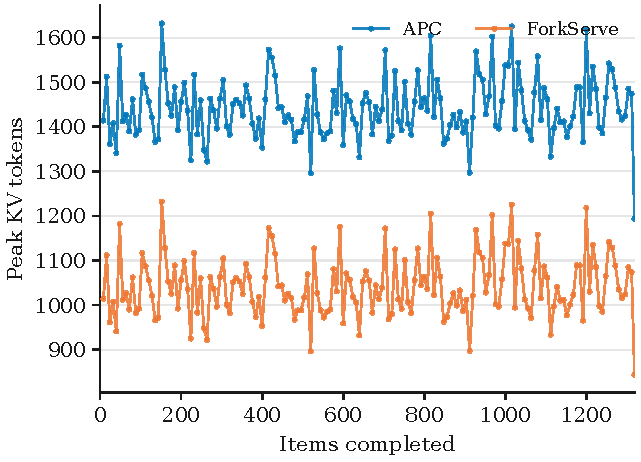
\includegraphics[width=\linewidth]{fig/peak_scatter_fs_vs_apc.pdf}
\end{minipage}\hfill
\begin{minipage}{0.49\textwidth}
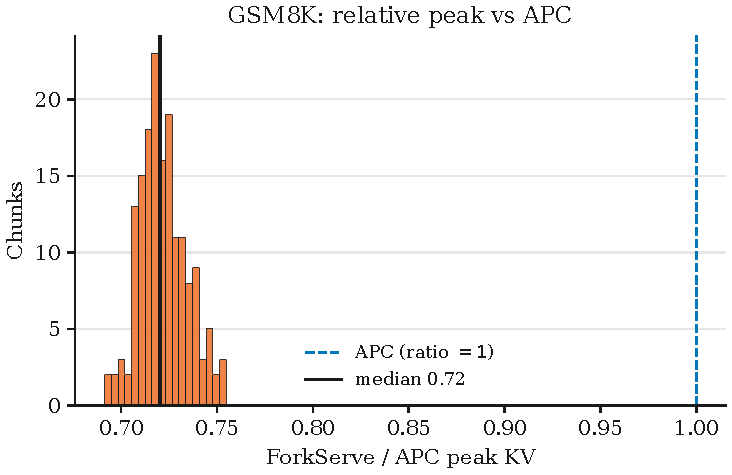
\includegraphics[width=\linewidth]{fig/peak_ratio_hist.pdf}
\end{minipage}
\caption{Left: peak KV on each of the $165$ GSM8K batches in the run log (eight problems per batch).
Branch-aware abort keeps ForkServe below APC on every batch.
Right: ratio $\mathrm{peak}^{\mathrm{FS}}/\mathrm{peak}^{\mathrm{APC}}$, median $0.72$: $28\%$ less cache than hashed prefix reuse.}
\end{figure}

\begin{figure}[h]
\centering
\begin{minipage}{0.49\textwidth}
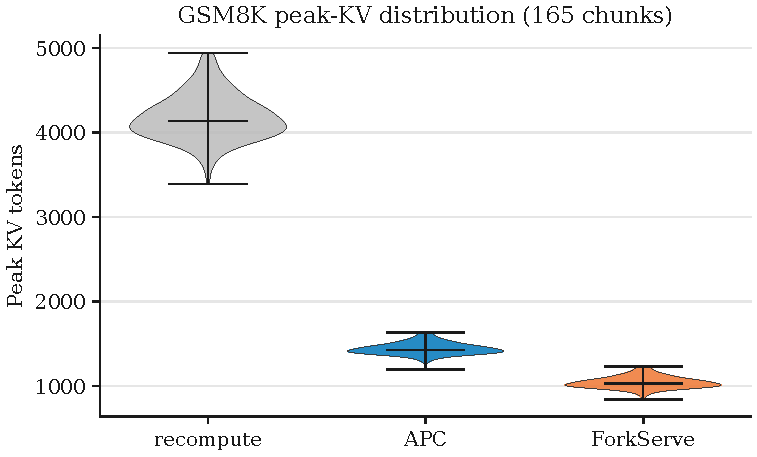
\includegraphics[width=\linewidth]{fig/peak_violin_gsm8k.pdf}
\end{minipage}\hfill
\begin{minipage}{0.49\textwidth}
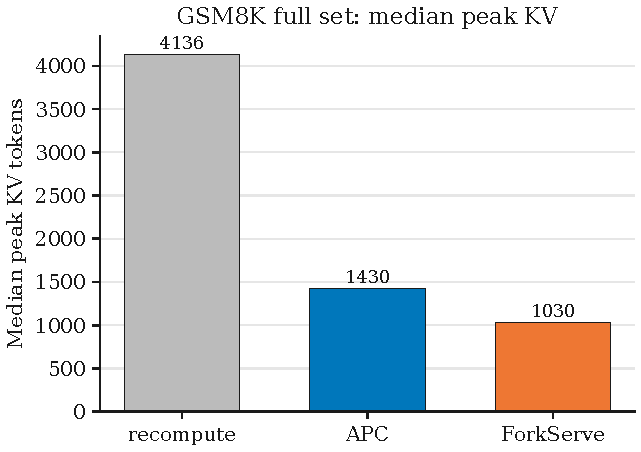
\includegraphics[width=\linewidth]{fig/peak_median_gsm8k.pdf}
\end{minipage}
\caption{Left: the storage gap versus APC is a shift of the whole distribution.
Right: median peak KV, $0.25\times$ recompute and $0.72\times$ APC.}
\end{figure}

\begin{table}[h]
\centering
\small
\begin{tabular}{@{}lrrrrrr@{}}
\toprule
Serving & accuracy & med $\mathrm{peak}$ & max $\mathrm{peak}$ & p95 $\mathrm{peak}$ & med fan-out & generate \\
\midrule
recompute & 0.847 (1117) & 4136 & 4944 & --- & $326\,\mathrm{ms}$ & $19.4\,\mathrm{min}$ \\
APC       & 0.844 (1113) & 1430 & 1632 & 1572 & $87\,\mathrm{ms}$  & $18.6\,\mathrm{min}$ \\
ForkServe & \textbf{0.845 (1114)} & \textbf{1030} & \textbf{1232} & \textbf{1172} & $140\,\mathrm{ms}$ & $18.9\,\mathrm{min}$ \\
\bottomrule
\end{tabular}
\caption{GSM8K, $n{=}1319$, $k{=}4$, $\mathrm{tp}{=}2$, eight problems per batch.
Storage (peak KV) is the ForkServe gain; accuracy and generate time stay with APC.}
\end{table}

\begin{table}[h]
\centering
\small
\begin{tabular}{@{}lcccc@{}}
\toprule
 & FS / APC & FS / rec. & batches FS${<}$APC & rec.\ $\gamma{=}0.20$ \\
\midrule
median $\mathrm{peak}$ & $1030/1430{=}0.720$ & $1030/4136{=}0.249$ & $165/165$ & $0.249\le 0.80$ \\
saving $S$ & $28\%$ & $75\%$ & --- & meets $\gamma$ \\
max $\mathrm{peak}$ & $1232$ vs.\ $1632$ & $1232$ vs.\ $4944$ & --- & --- \\
\bottomrule
\end{tabular}
\caption{Storage savings against both vLLM baselines.
$S_{\mathrm{APC}}{=}1-\mathrm{med}(\mathrm{peak}^{\mathrm{FS}})/\mathrm{med}(\mathrm{peak}^{\mathrm{APC}})$.
APC already removed most of the cloned-trunk cost ($1430$ vs.\ $4136$).
The extra $28\%$ is branch-aware abort: hashed union versus committed path.}
\end{table}

APC already avoids most of $M_{\mathrm{clone}}$.
ForkServe reduces the rest because abort frees unused residuals, leaving $M_{\mathrm{spine}}$ rather than the hashed union.
Every aligned batch satisfies $\mathrm{peak}^{\mathrm{FS}}<\mathrm{peak}^{\mathrm{APC}}$, so $\Delta>0$ holds throughout the test set: branch-aware sharing is storage-efficient on the full file.

\subsection{Quality}

\begin{figure}[h]
\centering
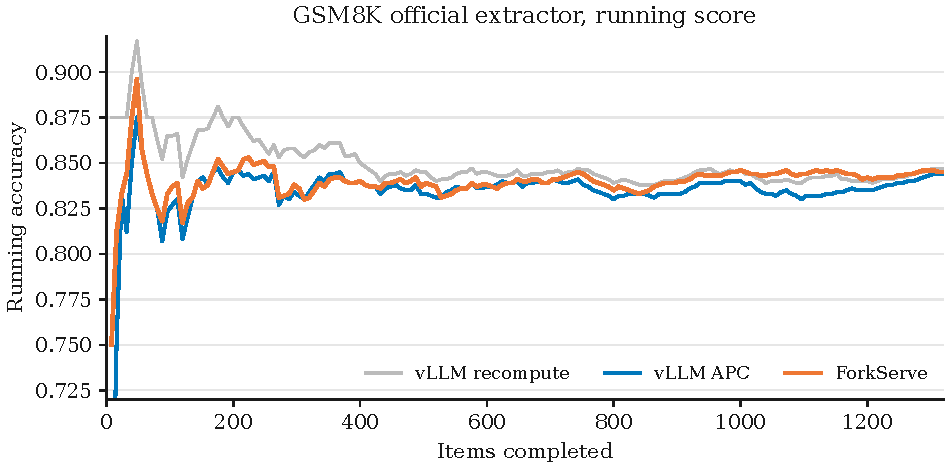
\includegraphics[width=\textwidth]{fig/accuracy_running_gsm8k.pdf}
\caption{\label{fig:acc}Official GSM8K extractor, running accuracy.
Tree-of-Thoughts accuracy ($\approx 0.845$) is below single-path generation ($\approx 0.941$) because several thoughts compete.
The committed path after abort is the same winner decode as APC, so scores stay aligned.}
\end{figure}

Running accuracy of recompute, APC, and ForkServe stays in $[0.83,0.85]$ (Figure~\ref{fig:acc}); the final correct counts differ by one to three problems.

\subsection{End-to-end latency}

Fan-out is a local prefill step.
ForkServe pays copy-on-write, residual flush, and abort on top of $W_{\mathrm{FS}}=L+\sum_i\ell_i$, so median $T_{\mathrm{fan}}$ is $140\,\mathrm{ms}$ versus $87\,\mathrm{ms}$ for APC and $326\,\mathrm{ms}$ for recompute.
That gap is the KV path, not extra tokens in $W$ versus APC.

Global latency is
\begin{equation}
T_{\mathrm{e2e}}
  \approx T_{\mathrm{fan}}+T_{\mathrm{dec}}(D),
\qquad D{=}512 \text{ on GSM8K.}
\end{equation}
$T_{\mathrm{dec}}$ is more than $95\%$ of $T_{\mathrm{e2e}}$.
On the full test set, generate time is $18.9\,\mathrm{min}$ (ForkServe), $18.6\,\mathrm{min}$ (APC), $19.4\,\mathrm{min}$ (recompute): the $53\,\mathrm{ms}$ extra fan-out per batch is $23\,\mathrm{s}$ in $\approx 1130\,\mathrm{s}$.
On the four-problem slices, ForkServe $T_{\mathrm{e2e}}$ is below APC on Tree-of-Thoughts (GSM8K $6992$ vs.\ $7011\,\mathrm{ms}$, Game24 $3558$ vs.\ $3583\,\mathrm{ms}$) and matches APC on HumanEval TTFT ($3568$ vs.\ $3566\,\mathrm{ms}$).
With $M_{\mathrm{spine}}<M_{\mathrm{APC}}$, $C\propto\mathrm{HBM}/M$ is larger, so $\Theta\propto C/T_{\mathrm{e2e}}$ is the storage-efficient serving optimum under a fixed GPU budget: ForkServe.

\begin{table}[h]
\centering
\small
\begin{tabular}{@{}lrrrr@{}}
\toprule
 & min & median & p95 & max \\
\midrule
recompute & $270$ & $326$ & $371$ & $392$ \\
APC & $75$ & $87$ & $95$ & $101$ \\
ForkServe & $122$ & $140$ & $152$ & $159$ \\
\bottomrule
\end{tabular}
\caption{Fan-out (ms) per GSM8K batch.
The $140$ vs.\ $87$ median is abort and copy-on-write against matched $W$; the storage-efficient claim is peak KV, not this micro-step.}
\end{table}

\begin{table}[h]
\centering
\small
\begin{tabular}{@{}lcccc@{}}
\toprule
 & med fan-out & generate wall-clock & vs.\ APC e2e & decode share of e2e \\
\midrule
recompute & $326\,\mathrm{ms}$ & $19.4\,\mathrm{min}$ & $+4.3\%$ & --- \\
APC & $87\,\mathrm{ms}$ & $18.6\,\mathrm{min}$ & --- & $1075/1102\,\mathrm{s}$ \\
ForkServe & $140\,\mathrm{ms}$ & $18.9\,\mathrm{min}$ & $+1.6\%$ & fan-out $23\,\mathrm{s}$ of $\approx 1130\,\mathrm{s}$ \\
\bottomrule
\end{tabular}
\caption{Generate time on full GSM8K.
Decode of $D{=}512$ sets the global $T_{\mathrm{e2e}}$; ForkServe stays with APC while $M$ is lower, which is storage-efficient serving in \eqref{eq:conc}.}
\end{table}

\section{Four-problem slices (settings B and C)}

Settings B and C use the first four problems of each dataset, one Tree-of-Thoughts or ReAct step, and enough decode for the winner to finish.
B is $\mathrm{tp}{=}2$ on GPU $0,1$ ($38497$\,MiB $\times 2$).
C is $\mathrm{tp}{=}4$ on GPU $0$--$3$ ($38797$\,MiB $\times 4$).
Peak follows the committed path after abort, so settings B and C share that storage footprint; latency follows $\mathrm{tp}$.
On GSM8K under C, APC scored $1.00$ and ForkServe $0.75$ on four items; accuracy is taken from the full test set (setting A).

\begin{figure}[h]
\centering
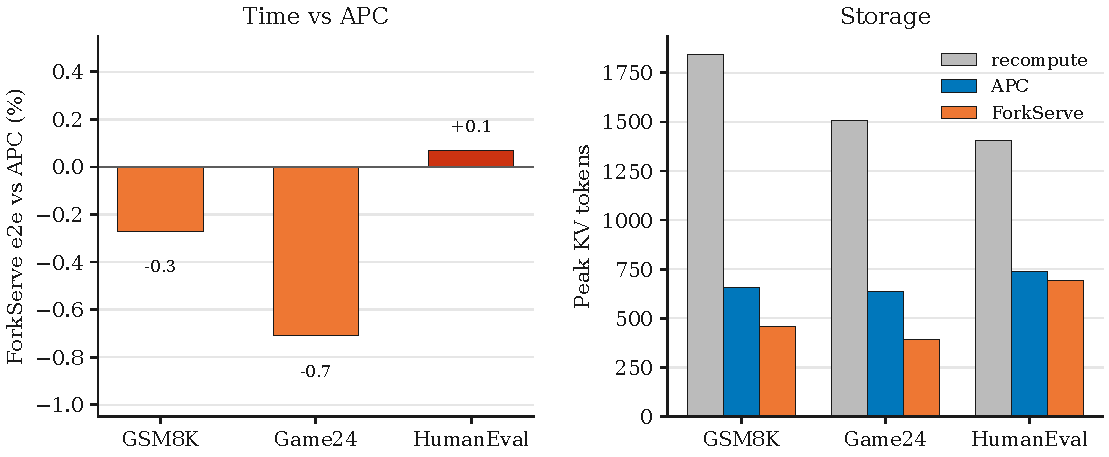
\includegraphics[width=\textwidth]{fig/rl3_lat_tp2.pdf}
\caption{Setting B ($\mathrm{tp}{=}2$, $n{=}4$).
Left: end-to-end time stays with APC ($-0.3\%$, $-0.7\%$, $+0.1\%$) because decode dominates $T_{\mathrm{e2e}}$.
Right: peak resident KV on the same runs.
Branch-aware abort compresses storage to $M_{\mathrm{spine}}$ ($0.70\times$, $0.61\times$, $0.94\times$ APC) at stable latency.}
\end{figure}

\subsection{GSM8K (settings B and C)}

Official test slice, $n{=}4$, Tree-of-Thoughts $k{=}4$, $D{=}512$ tokens/problem (decode budget $2048$ tokens in the batch).
Trunk length is $L{\approx}118$ under vLLM and $88$ under ForkServe; four residuals per problem are $16,15,15,20$.

\begin{table}[h]
\centering
\small
\begin{tabular}{@{}clrrrr@{}}
\toprule
$\mathrm{tp}$ & Serving & $\mathrm{peak}$ & fan-out (ms) & e2e (ms) & decode (ms) \\
\midrule
2 & recompute & 1844 & 191 & 7103 & 6912 \\
2 & APC & 659 & 60 & 7011 & 6885 \\
2 & ForkServe & 459 & 93 & 6992 & 6898 \\
4 & recompute & 1844 & 114 & 4353 & 4238 \\
4 & APC & 659 & 43 & 4308 & 4229 \\
4 & ForkServe & 459 & 58 & 4292 & 4234 \\
\bottomrule
\end{tabular}
\caption{GSM8K, $n{=}4$.
FS/APC peak ${=}0.70$; FS/recompute ${=}0.25$: branch-aware sharing is storage-efficient at both $\mathrm{tp}{=}2$ and $\mathrm{tp}{=}4$.
End-to-end vs.\ APC is $-0.3\%$ at $\mathrm{tp}{=}2$ and $-0.4\%$ at $\mathrm{tp}{=}4$.}
\end{table}

\subsection{Game24 (settings B and C)}

\texttt{24.csv} slice, $n{=}4$, Tree-of-Thoughts $k{=}4$, $D{=}256$ tokens/problem.
$L{=}72$; residuals $25,24,21,17$.
The trunk is shorter than GSM8K, so $M_{\mathrm{spine}}/M_{\mathrm{APC}}$ is lower ($0.61$) because unused residuals are a larger share of the hashed union.

\begin{table}[h]
\centering
\small
\begin{tabular}{@{}clrrrrc@{}}
\toprule
$\mathrm{tp}$ & Serving & $\mathrm{peak}$ & fan-out (ms) & e2e (ms) & decode (ms) & success \\
\midrule
2 & recompute & 1508 & 140 & 3638 & 3498 & $1.00$ \\
2 & APC & 638 & 63 & 3583 & 3476 & $1.00$ \\
2 & ForkServe & 390 & 79 & 3558 & 3479 & $1.00$ \\
4 & recompute & 1508 & 102 & 2246 & 2144 & $1.00$ \\
4 & APC & 638 & 47 & 2234 & 2133 & $1.00$ \\
4 & ForkServe & 390 & 53 & 2188 & 2134 & $1.00$ \\
\bottomrule
\end{tabular}
\caption{Game24, $n{=}4$.
FS/APC peak ${=}0.61$; FS/recompute ${=}0.26$.
A short trunk raises the unused-residual share, so storage-efficient abort saves more versus APC than on GSM8K.
End-to-end vs.\ APC is $-0.7\%$ at $\mathrm{tp}{=}2$ and $-2.0\%$ at $\mathrm{tp}{=}4$.
Success matches on all four problems.}
\end{table}

\subsection{HumanEval (settings B and C)}

Official HumanEval slice, $n{=}4$, ReAct wrap+recovery $k{=}2$, $D{=}256$, idle $2000\,\mathrm{ms}$, then wrap+observation decode.
Latency is time-to-first-token after the observation.
$L{\approx}180$ (vLLM) / $174$ (ForkServe); wrap and recovery residuals are short ($7,11$), then a long observation suffix (up to $321$ tokens).
With $k{=}2$ and a long suffix, \eqref{eq:gap} gives FS/APC peak $0.94$.

\begin{table}[h]
\centering
\small
\begin{tabular}{@{}clrrrrc@{}}
\toprule
$\mathrm{tp}$ & Serving & $\mathrm{peak}$ & fan-out (ms) & e2e (ms) & TTFT (ms) & pass@1 \\
\midrule
2 & recompute & 1406 & 141 & 3787 & 3646 & $0.75$ \\
2 & APC & 739 & 39 & 3682 & 3566 & $0.75$ \\
2 & ForkServe & 695 & 76 & 3645 & 3568 & $0.75$ \\
4 & recompute & 1406 & 83 & 2342 & 2259 & $0.75$ \\
4 & APC & 739 & 28 & 2302 & 2227 & $0.75$ \\
4 & ForkServe & 695 & 49 & 2287 & 2236 & $0.75$ \\
\bottomrule
\end{tabular}
\caption{HumanEval, $n{=}4$.
FS/APC peak ${=}0.94$; FS/recompute ${=}0.49$.
ReAct $k{=}2$ with a long observation suffix leaves less unused KV, so the storage gap versus APC is smaller, as \eqref{eq:gap} predicts.
TTFT vs.\ APC is $+0.1\%$ at $\mathrm{tp}{=}2$ and $+0.4\%$ at $\mathrm{tp}{=}4$.
Pass@1 matches APC ($3/4$).}
\end{table}

\begin{figure}[h]
\centering
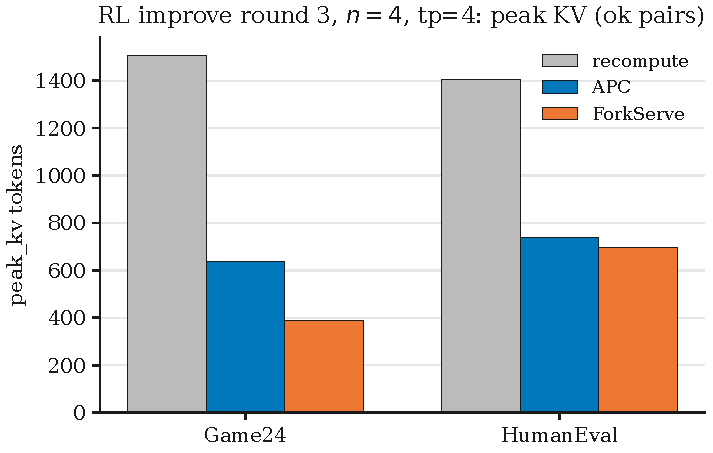
\includegraphics[width=0.72\textwidth]{fig/rl3_peak_tp4_ok.pdf}
\caption{Setting C ($\mathrm{tp}{=}4$): Game24 and HumanEval.
$\mathrm{peak}^{\mathrm{FS}}/\mathrm{peak}^{\mathrm{APC}}$ is $0.61$ and $0.94$, as in setting B.
Those storage ratios are fixed by $k$ and the residuals after abort (\eqref{eq:gap}).
Four-way tensor parallel shards the same committed path, so the HBM advantage versus APC is a property of branch-aware sharing and applies at $\mathrm{tp}{=}4$.}
\end{figure}

\subsection{Tensor parallel B versus C}

\begin{table}[h]
\centering
\small
\begin{tabular}{@{}lcccc@{}}
\toprule
Dataset & $\mathrm{peak}$ (tokens) & e2e FS, $\mathrm{tp}{=}2$ & e2e FS, $\mathrm{tp}{=}4$ & $\mathrm{tp}{=}4/\mathrm{tp}{=}2$ \\
\midrule
GSM8K & 459 & $6992\,\mathrm{ms}$ & $4292\,\mathrm{ms}$ & $0.61$ \\
Game24 & 390 & $3558\,\mathrm{ms}$ & $2188\,\mathrm{ms}$ & $0.61$ \\
HumanEval (TTFT) & 695 & $3568\,\mathrm{ms}$ & $2236\,\mathrm{ms}$ & $0.63$ \\
\bottomrule
\end{tabular}
\caption{From $\mathrm{tp}{=}2$ to $\mathrm{tp}{=}4$, ForkServe latency (TTFT on HumanEval) scales by $0.61$--$0.63$, in line with decode on twice as many ranks.
Peak is the committed-path length $M_{\mathrm{spine}}$, so the storage ratio to APC is already set by abort in setting B.
Four-GPU decode therefore stacks with that storage efficiency: each tree occupies less cache than APC, and $C\propto\mathrm{HBM}/M$ is larger.}
\end{table}

Tree-of-Thoughts ($k{=}4$) gives $\mathrm{peak}^{\mathrm{FS}}/\mathrm{peak}^{\mathrm{APC}}\in[0.61,0.70]$, close to setting A on GSM8K ($0.72$).
ReAct ($k{=}2$) gives $0.94$.

\section{Qwen3-14B math suite (settings G and H)}

Settings G and H repeat the APC vs.\ ForkServe recipe of E and F on Qwen3-14B:
the same seven files, $k{=}4$, batches of eight, $D{\in}\{512,768\}$, $\mathrm{tp}{=}2$ then $\mathrm{tp}{=}4$.
Peak KV matches the 8B suite token-for-token: the trunks and residuals are the same strings, so $M_{\mathrm{spine}}$ does not depend on width.

Resident memory is $\approx 37381$--$37515$\,MiB/rank (APC) and $37515$--$37733$\,MiB (ForkServe) at $\mathrm{tp}{=}2$,
and $\approx 37691$--$37711$ / $37813$--$37871$\,MiB at $\mathrm{tp}{=}4$.

\subsection{Accuracy comparison}

\begin{table}[h]
\centering
\small
\resizebox{\textwidth}{!}{%
\begin{tabular}{@{}lrrcccccc@{}}
\toprule
 & & & \multicolumn{3}{c}{$\mathrm{tp}{=}2$ (G)} & \multicolumn{3}{c}{$\mathrm{tp}{=}4$ (H)} \\
\cmidrule(lr){4-6}\cmidrule(lr){7-9}
Dataset & $n$ & $D$ & APC & FS & $\Delta$ & APC & FS & $\Delta$ \\
\midrule
GSM8K    & $80$ & $512$ & $\mathbf{0.825}$ ($66$) & $0.813$ ($65$) & $-1.3$\,pp & $0.788$ ($63$) & $\mathbf{0.838}$ ($67$) & $+5.0$\,pp \\
SVAMP    & $80$ & $512$ & $\mathbf{0.825}$ ($66$) & $0.813$ ($65$) & $-1.3$\,pp & $\mathbf{0.813}$ ($65$) & $0.800$ ($64$) & $-1.3$\,pp \\
GSM-Hard & $80$ & $512$ & $0.663$ ($53$) & $0.663$ ($53$) & $0$ & $\mathbf{0.663}$ ($53$) & $0.613$ ($49$) & $-5.0$\,pp \\
MATH-500 & $80$ & $768$ & $0.563$ ($45$) & $\mathbf{0.588}$ ($47$) & $+2.5$\,pp & $\mathbf{0.650}$ ($52$) & $0.588$ ($47$) & $-6.3$\,pp \\
AIME     & $73$ & $768$ & $0.027$ ($2$)  & $\mathbf{0.041}$ ($3$)  & $+1.4$\,pp & $\mathbf{0.041}$ ($3$)  & $0.027$ ($2$)  & $-1.4$\,pp \\
AMC23    & $40$ & $768$ & $0.325$ ($13$) & $0.325$ ($13$) & $0$ & $\mathbf{0.300}$ ($12$) & $0.250$ ($10$) & $-5.0$\,pp \\
Game24   & $80$ & $512$ & $0.725$ ($58$) & $\mathbf{0.750}$ ($60$) & $+2.5$\,pp & $0.688$ ($55$) & $\mathbf{0.713}$ ($57$) & $+2.5$\,pp \\
\midrule
All $513$ & $513$ & --- & $0.591$ ($303$) & $\mathbf{0.596}$ ($306$) & $+0.6$\,pp & $\mathbf{0.591}$ ($303$) & $0.577$ ($296$) & $-1.4$\,pp \\
\bottomrule
\end{tabular}%
}
\caption{Qwen3-14B official accuracy, APC vs.\ ForkServe.
The pool is $513$ items.
At two GPUs ForkServe is $+3$ problems; at four GPUs $-7$.
No file differs by more than five problems.
AIME remains $2$--$3/73$ on both stacks.}
\end{table}

\begin{figure}[h]
\centering
\begin{tikzpicture}[x=1.38cm,y=2.45cm]
  \def\bw{0.16}
  \foreach \y in {0.0,0.25,0.50,0.75,1.00} {
    \draw[Rule] (-0.55,\y) -- (7.05,\y);
    \node[font=\scriptsize,Mute,anchor=east] at (-0.62,\y) {\y};
  }
  \foreach \i/\lab/\atwo/\ftwo/\afour/\ffour in {
    0/GSM8K/0.825/0.8125/0.7875/0.8375,
    1/SVAMP/0.825/0.8125/0.8125/0.800,
    2/GSM-H/0.6625/0.6625/0.6625/0.6125,
    3/MATH/0.5625/0.5875/0.650/0.5875,
    4/AIME/0.0274/0.0411/0.0411/0.0274,
    5/AMC23/0.325/0.325/0.300/0.250,
    6/G24/0.725/0.750/0.6875/0.7125} {
    \fill[APC]  ({\i-1.5*\bw-\bw},0) rectangle ({\i-0.5*\bw-\bw},\atwo);
    \fill[FS]   ({\i-0.5*\bw-\bw},0) rectangle ({\i-0.5*\bw},\ftwo);
    \fill[APCp] ({\i-0.5*\bw},0) rectangle ({\i+0.5*\bw},\afour);
    \fill[FSp]  ({\i+0.5*\bw},0) rectangle ({\i+1.5*\bw},\ffour);
    \node[font=\scriptsize,anchor=east,rotate=40] at (\i,-0.04) {\lab};
  }
  \draw[Ink] (-0.55,0) -- (7.05,0);
  \fill[APC] (0.05,1.12) rectangle (0.28,1.20);
  \node[font=\scriptsize,anchor=west] at (0.32,1.16) {APC $\mathrm{tp}{=}2$};
  \fill[FS] (2.05,1.12) rectangle (2.28,1.20);
  \node[font=\scriptsize,anchor=west] at (2.32,1.16) {FS $\mathrm{tp}{=}2$};
  \fill[APCp] (3.85,1.12) rectangle (4.08,1.20);
  \node[font=\scriptsize,anchor=west] at (4.12,1.16) {APC $\mathrm{tp}{=}4$};
  \fill[FSp] (5.75,1.12) rectangle (5.98,1.20);
  \node[font=\scriptsize,anchor=west] at (6.02,1.16) {FS $\mathrm{tp}{=}4$};
  \node[font=\small,anchor=south] at (3.2,1.24) {Official accuracy, Qwen3-14B};
\end{tikzpicture}
\caption{Qwen3-14B accuracy, four stacks on each file.
Orange tracks blue; the largest gaps are MATH-500 and GSM-Hard at $\mathrm{tp}{=}4$ (five problems).}
\end{figure}

\subsection{System metrics}

\begin{table}[h]
\centering
\small
\resizebox{\textwidth}{!}{%
\begin{tabular}{@{}lrrrrrrrrr@{}}
\toprule
 & \multicolumn{3}{c}{Peak KV (tokens)} & \multicolumn{3}{c}{e2e (s), $\mathrm{tp}{=}2$} & \multicolumn{3}{c}{e2e (s), $\mathrm{tp}{=}4$} \\
\cmidrule(lr){2-4}\cmidrule(lr){5-7}\cmidrule(lr){8-10}
Dataset & APC & FS & FS/APC & APC & FS & vs.\ APC & APC & FS & vs.\ APC \\
\midrule
GSM8K    & $1582$ & $\mathbf{1182}$ & $0.75$ & $72.3$ & $72.0$ & $-0.5\%$ & $44.6$ & $44.0$ & $-1.3\%$ \\
SVAMP    & $1359$ & $\mathbf{959}$  & $0.71$ & $56.6$ & $53.6$ & $-5.3\%$ & $34.6$ & $34.3$ & $-0.8\%$ \\
GSM-Hard & $1462$ & $\mathbf{1062}$ & $0.73$ & $72.9$ & $71.6$ & $-1.8\%$ & $43.9$ & $44.8$ & $+2.1\%$ \\
MATH-500 & $1765$ & $\mathbf{1349}$ & $0.76$ & $110.6$ & $110.1$ & $-0.4\%$ & $67.4$ & $67.5$ & $+0.1\%$ \\
AIME     & $2118$ & $\mathbf{1702}$ & $0.80$ & $111.1$ & $110.8$ & $-0.3\%$ & $68.0$ & $68.0$ & $0.0\%$ \\
AMC23    & $1920$ & $\mathbf{1504}$ & $0.78$ & $55.9$ & $55.7$ & $-0.4\%$ & $34.0$ & $34.0$ & $-0.1\%$ \\
Game24   & $1289$ & $\mathbf{793}$  & $0.62$ & $74.2$ & $74.0$ & $-0.3\%$ & $45.4$ & $45.1$ & $-0.7\%$ \\
\bottomrule
\end{tabular}%
}
\caption{Qwen3-14B storage and generate time.
Peak KV equals the 8B suite and is independent of $\mathrm{tp}$.
Wall-clock is within $3\%$ of APC except SVAMP at two GPUs ($-5.3\%$), where ForkServe emits fewer winner tokens.}
\end{table}

\begin{table}[h]
\centering
\small
\resizebox{\textwidth}{!}{%
\begin{tabular}{@{}lrrrrrrrrr@{}}
\toprule
 & \multicolumn{4}{c}{Fan-out (s)} & \multicolumn{2}{c}{Decode tokens, $\mathrm{tp}{=}2$} & \multicolumn{2}{c}{Decode tokens, $\mathrm{tp}{=}4$} \\
\cmidrule(lr){2-5}\cmidrule(lr){6-7}\cmidrule(lr){8-9}
Dataset & APC t2 & FS t2 & APC t4 & FS t4 & APC & FS & APC & FS \\
\midrule
GSM8K    & $0.89$ & $1.41$ & $0.60$ & $0.93$ & $40960$ & $23576$ & $40960$ & $22586$ \\
SVAMP    & $0.87$ & $1.30$ & $0.58$ & $0.82$ & $40960$ & $17139$ & $40960$ & $16840$ \\
GSM-Hard & $0.84$ & $1.22$ & $0.56$ & $0.83$ & $40960$ & $26555$ & $40960$ & $27417$ \\
MATH-500 & $0.90$ & $1.41$ & $0.60$ & $0.92$ & $61440$ & $47465$ & $61440$ & $47693$ \\
AIME     & $0.87$ & $1.56$ & $0.58$ & $1.01$ & $56064$ & $55758$ & $56064$ & $55758$ \\
AMC23    & $0.47$ & $0.78$ & $0.31$ & $0.51$ & $30720$ & $29487$ & $30720$ & $29417$ \\
Game24   & $1.06$ & $1.28$ & $0.69$ & $0.82$ & $40960$ & $35824$ & $40960$ & $36358$ \\
\bottomrule
\end{tabular}%
}
\caption{Qwen3-14B fan-out and winner decode tokens.
Fan-out is $1.2$--$1.9\times$ APC and still $<3\%$ of $T_{\mathrm{e2e}}$.
APC always spends the decode budget; ForkServe stops early on GSM8K and SVAMP.}
\end{table}

\begin{table}[h]
\centering
\small
\begin{tabular}{@{}lcccccc@{}}
\toprule
Dataset & FS e2e t2 (s) & FS e2e t4 (s) & $4/2$ & APC e2e $4/2$ & peak FS/APC & dec.\ share \\
\midrule
GSM8K    & $72.0$ & $44.0$ & $0.61$ & $0.62$ & $0.75$ & $0.98$ \\
SVAMP    & $53.6$ & $34.3$ & $0.64$ & $0.61$ & $0.71$ & $0.98$ \\
GSM-Hard & $71.6$ & $44.8$ & $0.63$ & $0.60$ & $0.73$ & $0.98$ \\
MATH-500 & $110.1$ & $67.5$ & $0.61$ & $0.61$ & $0.76$ & $0.99$ \\
AIME     & $110.8$ & $68.0$ & $0.61$ & $0.61$ & $0.80$ & $0.99$ \\
AMC23    & $55.7$ & $34.0$ & $0.61$ & $0.61$ & $0.78$ & $0.99$ \\
Game24   & $74.0$ & $45.1$ & $0.61$ & $0.61$ & $0.62$ & $0.98$ \\
\bottomrule
\end{tabular}
\caption{Qwen3-14B tensor-parallel scaling (ForkServe).
Four ranks cut wall-clock by $0.61$--$0.64$, in line with setting C on the same weights.
Peak is unchanged.
Decode share of e2e is $0.98$--$0.99$.}
\end{table}

\begin{figure}[h]
\centering
\begin{tikzpicture}[x=1.22cm,y=0.00112cm]
  \def\w{0.34}
  \foreach \y in {0,500,1000,1500,2000} {
    \draw[Rule] (-0.45,\y) -- (6.85,\y);
    \node[font=\scriptsize,Mute,anchor=east] at (-0.52,\y) {\y};
  }
  \foreach \i/\lab/\apc/\fs in {
    0/GSM8K/1582/1182,
    1/SVAMP/1359/959,
    2/GSM-H/1462/1062,
    3/MATH/1765/1349,
    4/AIME/2118/1702,
    5/AMC23/1920/1504,
    6/G24/1289/793} {
    \fill[APC] ({\i-\w},0) rectangle ({\i},\apc);
    \fill[FS] ({\i},0) rectangle ({\i+\w},\fs);
    \node[font=\scriptsize,anchor=east,rotate=40] at (\i,-50) {\lab};
  }
  \draw[Ink] (-0.45,0) -- (6.85,0);
  \fill[APC] (4.35,2280) rectangle (4.58,2480);
  \node[font=\scriptsize,anchor=west] at (4.64,2380) {APC};
  \fill[FS] (5.45,2280) rectangle (5.68,2480);
  \node[font=\scriptsize,anchor=west] at (5.74,2380) {ForkServe};
  \node[font=\small,anchor=south] at (3.2,2580) {Peak resident KV (tokens), Qwen3-14B};
\end{tikzpicture}
\caption{Qwen3-14B peak KV, shared by settings G and H.
The bars equal the 8B figure: storage is $M_{\mathrm{spine}}$, not model width.}
\end{figure}

\begin{figure}[h]
\centering
\begin{tikzpicture}[x=1.38cm,y=0.022cm]
  \def\bw{0.16}
  \foreach \y in {0,30,60,90,120} {
    \draw[Rule] (-0.55,\y) -- (7.05,\y);
    \node[font=\scriptsize,Mute,anchor=east] at (-0.62,\y) {\y};
  }
  \foreach \i/\lab/\atwo/\ftwo/\afour/\ffour in {
    0/GSM8K/72.3/72.0/44.6/44.0,
    1/SVAMP/56.6/53.6/34.6/34.3,
    2/GSM-H/72.9/71.6/43.9/44.8,
    3/MATH/110.6/110.1/67.4/67.5,
    4/AIME/111.1/110.8/68.0/68.0,
    5/AMC23/55.9/55.7/34.0/34.0,
    6/G24/74.2/74.0/45.4/45.1} {
    \fill[APC]  ({\i-1.5*\bw-\bw},0) rectangle ({\i-0.5*\bw-\bw},\atwo);
    \fill[FS]   ({\i-0.5*\bw-\bw},0) rectangle ({\i-0.5*\bw},\ftwo);
    \fill[APCp] ({\i-0.5*\bw},0) rectangle ({\i+0.5*\bw},\afour);
    \fill[FSp]  ({\i+0.5*\bw},0) rectangle ({\i+1.5*\bw},\ffour);
    \node[font=\scriptsize,anchor=east,rotate=40] at (\i,-3.2) {\lab};
  }
  \draw[Ink] (-0.55,0) -- (7.05,0);
  \fill[APC] (0.05,118) rectangle (0.28,126);
  \node[font=\scriptsize,anchor=west] at (0.32,122) {APC $\mathrm{tp}{=}2$};
  \fill[FS] (2.05,118) rectangle (2.28,126);
  \node[font=\scriptsize,anchor=west] at (2.32,122) {FS $\mathrm{tp}{=}2$};
  \fill[APCp] (3.85,118) rectangle (4.08,126);
  \node[font=\scriptsize,anchor=west] at (4.12,122) {APC $\mathrm{tp}{=}4$};
  \fill[FSp] (5.75,118) rectangle (5.98,126);
  \node[font=\scriptsize,anchor=west] at (6.02,122) {FS $\mathrm{tp}{=}4$};
  \node[font=\small,anchor=south] at (3.2,132) {Generate wall-clock (s), Qwen3-14B};
\end{tikzpicture}
\caption{Qwen3-14B end-to-end generate time.
Orange sits on blue in each tensor-width pair.
Light bars ($\mathrm{tp}{=}4$) are $0.61$--$0.64\times$ the dark bars.}
\end{figure}

\begin{figure}[h]
\centering
\begin{tikzpicture}[x=1.38cm,y=1.35cm]
  \def\bw{0.16}
  \foreach \y in {0.0,0.5,1.0,1.5} {
    \draw[Rule] (-0.55,\y) -- (7.05,\y);
    \node[font=\scriptsize,Mute,anchor=east] at (-0.62,\y) {\y};
  }
  \foreach \i/\lab/\atwo/\ftwo/\afour/\ffour in {
    0/GSM8K/0.89/1.41/0.60/0.93,
    1/SVAMP/0.87/1.30/0.58/0.82,
    2/GSM-H/0.84/1.22/0.56/0.83,
    3/MATH/0.90/1.41/0.60/0.92,
    4/AIME/0.87/1.56/0.58/1.01,
    5/AMC23/0.47/0.78/0.31/0.51,
    6/G24/1.06/1.28/0.69/0.82} {
    \fill[APC]  ({\i-1.5*\bw-\bw},0) rectangle ({\i-0.5*\bw-\bw},\atwo);
    \fill[FS]   ({\i-0.5*\bw-\bw},0) rectangle ({\i-0.5*\bw},\ftwo);
    \fill[APCp] ({\i-0.5*\bw},0) rectangle ({\i+0.5*\bw},\afour);
    \fill[FSp]  ({\i+0.5*\bw},0) rectangle ({\i+1.5*\bw},\ffour);
    \node[font=\scriptsize,anchor=east,rotate=40] at (\i,-0.08) {\lab};
  }
  \draw[Ink] (-0.55,0) -- (7.05,0);
  \fill[APC] (0.05,1.72) rectangle (0.28,1.82);
  \node[font=\scriptsize,anchor=west] at (0.32,1.77) {APC $\mathrm{tp}{=}2$};
  \fill[FS] (2.05,1.72) rectangle (2.28,1.82);
  \node[font=\scriptsize,anchor=west] at (2.32,1.77) {FS $\mathrm{tp}{=}2$};
  \fill[APCp] (3.85,1.72) rectangle (4.08,1.82);
  \node[font=\scriptsize,anchor=west] at (4.12,1.77) {APC $\mathrm{tp}{=}4$};
  \fill[FSp] (5.75,1.72) rectangle (5.98,1.82);
  \node[font=\scriptsize,anchor=west] at (6.02,1.77) {FS $\mathrm{tp}{=}4$};
  \node[font=\small,anchor=south] at (3.2,1.88) {Fan-out (s), Qwen3-14B};
\end{tikzpicture}
\caption{Qwen3-14B fan-out.
The abort/CoW tax is larger in milliseconds than on 8B, but still tenths of a second against $34$--$111\,\mathrm{s}$ generate.}
\end{figure}

\section{Qwen3-8B math suite (settings E and F)}

Settings E and F run the same APC vs.\ ForkServe recipe on Qwen3-8B:
Tree-of-Thoughts $k{=}4$, batches of eight, GPU $0,1$ at $\mathrm{tp}{=}2$ (E) and GPU $0$--$3$ at $\mathrm{tp}{=}4$ (F).
Grade-school files (GSM8K, SVAMP, GSM-Hard, Game24) decode $D{=}512$; contest files (MATH-500, AIME, AMC23) decode $D{=}768$.
$n{=}80$ except AIME ($73$) and AMC23 ($40$).
There is no recompute arm: the comparison is hashed prefix reuse versus branch-aware abort.

Resident memory is $\approx 37305$\,MiB/rank (APC) and $37423$--$37579$\,MiB (ForkServe) at $\mathrm{tp}{=}2$,
and $\approx 37599$ / $37665$\,MiB at $\mathrm{tp}{=}4$.
Peak KV is identical across tensor widths: it is $M_{\mathrm{spine}}$, not a function of rank count.

\subsection{Accuracy comparison}

\begin{table}[h]
\centering
\small
\resizebox{\textwidth}{!}{%
\begin{tabular}{@{}lrrcccccc@{}}
\toprule
 & & & \multicolumn{3}{c}{$\mathrm{tp}{=}2$ (E)} & \multicolumn{3}{c}{$\mathrm{tp}{=}4$ (F)} \\
\cmidrule(lr){4-6}\cmidrule(lr){7-9}
Dataset & $n$ & $D$ & APC & FS & $\Delta$ & APC & FS & $\Delta$ \\
\midrule
GSM8K    & $80$ & $512$ & $0.925$ ($74$) & $\mathbf{0.963}$ ($77$) & $+3.8$\,pp & $0.925$ ($74$) & $\mathbf{0.950}$ ($76$) & $+2.5$\,pp \\
SVAMP    & $80$ & $512$ & $0.863$ ($69$) & $\mathbf{0.888}$ ($71$) & $+2.5$\,pp & $\mathbf{0.863}$ ($69$) & $0.838$ ($67$) & $-2.5$\,pp \\
GSM-Hard & $80$ & $512$ & $0.650$ ($52$) & $\mathbf{0.663}$ ($53$) & $+1.3$\,pp & $0.638$ ($51$) & $0.638$ ($51$) & $0$ \\
MATH-500 & $80$ & $768$ & $0.638$ ($51$) & $\mathbf{0.650}$ ($52$) & $+1.3$\,pp & $\mathbf{0.675}$ ($54$) & $0.638$ ($51$) & $-3.8$\,pp \\
AIME     & $73$ & $768$ & $0.041$ ($3$)  & $0.041$ ($3$)  & $0$        & $0.027$ ($2$)  & $\mathbf{0.041}$ ($3$)  & $+1.4$\,pp \\
AMC23    & $40$ & $768$ & $0.275$ ($11$) & $\mathbf{0.350}$ ($14$) & $+7.5$\,pp & $\mathbf{0.350}$ ($14$) & $0.300$ ($12$) & $-5.0$\,pp \\
Game24   & $80$ & $512$ & $\mathbf{0.713}$ ($57$) & $0.700$ ($56$) & $-1.3$\,pp & $\mathbf{0.688}$ ($55$) & $0.650$ ($52$) & $-3.8$\,pp \\
\midrule
All $513$ & $513$ & --- & $0.618$ ($317$) & $\mathbf{0.635}$ ($326$) & $+1.8$\,pp & $\mathbf{0.622}$ ($319$) & $0.608$ ($312$) & $-1.4$\,pp \\
\bottomrule
\end{tabular}%
}
\caption{Official accuracy, APC vs.\ ForkServe, $\mathrm{tp}{=}2$ and $\mathrm{tp}{=}4$.
Parentheses are correct counts.
The last row is micro-average over the union of the seven files ($5{\times}80+73+40{=}513$).
At two GPUs ForkServe is ahead on six files and on the pool ($+9$ problems).
At four GPUs the pool is within seven problems; no file differs by more than three.}
\end{table}

On GSM8K at $\mathrm{tp}{=}2$ the step slices stay with ForkServe:
steps $1$ $4/4$ vs.\ $4/4$,
steps $2$ $27/28$ vs.\ $26/28$,
steps $3$ $18/18$ vs.\ $17/18$,
steps $4{+}$ $28/30$ vs.\ $27/30$.
MATH-500 level $1$ is $7/8$ on both stacks.
AIME stays $2$--$3/73$: $8$B Tree-of-Thoughts with $D{=}768$ does not solve contest items, so that file is an efficiency check.

\begin{figure}[h]
\centering
\begin{tikzpicture}[x=1.38cm,y=2.45cm]
  \def\bw{0.16}
  \foreach \y in {0.0,0.25,0.50,0.75,1.00} {
    \draw[Rule] (-0.55,\y) -- (7.05,\y);
    \node[font=\scriptsize,Mute,anchor=east] at (-0.62,\y) {\y};
  }
  \foreach \i/\lab/\atwo/\ftwo/\afour/\ffour in {
    0/GSM8K/0.925/0.9625/0.925/0.950,
    1/SVAMP/0.8625/0.8875/0.8625/0.8375,
    2/GSM-H/0.650/0.6625/0.6375/0.6375,
    3/MATH/0.6375/0.650/0.675/0.6375,
    4/AIME/0.0411/0.0411/0.0274/0.0411,
    5/AMC23/0.275/0.350/0.350/0.300,
    6/G24/0.7125/0.700/0.6875/0.650} {
    \fill[APC]  ({\i-1.5*\bw-\bw},0) rectangle ({\i-0.5*\bw-\bw},\atwo);
    \fill[FS]   ({\i-0.5*\bw-\bw},0) rectangle ({\i-0.5*\bw},\ftwo);
    \fill[APCp] ({\i-0.5*\bw},0) rectangle ({\i+0.5*\bw},\afour);
    \fill[FSp]  ({\i+0.5*\bw},0) rectangle ({\i+1.5*\bw},\ffour);
    \node[font=\scriptsize,anchor=east,rotate=40] at (\i,-0.04) {\lab};
  }
  \draw[Ink] (-0.55,0) -- (7.05,0);
  \fill[APC] (0.05,1.12) rectangle (0.28,1.20);
  \node[font=\scriptsize,anchor=west] at (0.32,1.16) {APC $\mathrm{tp}{=}2$};
  \fill[FS] (2.05,1.12) rectangle (2.28,1.20);
  \node[font=\scriptsize,anchor=west] at (2.32,1.16) {FS $\mathrm{tp}{=}2$};
  \fill[APCp] (3.85,1.12) rectangle (4.08,1.20);
  \node[font=\scriptsize,anchor=west] at (4.12,1.16) {APC $\mathrm{tp}{=}4$};
  \fill[FSp] (5.75,1.12) rectangle (5.98,1.20);
  \node[font=\scriptsize,anchor=west] at (6.02,1.16) {FS $\mathrm{tp}{=}4$};
  \node[font=\small,anchor=south] at (3.2,1.24) {Official accuracy};
\end{tikzpicture}
\caption{Accuracy, four stacks on each file.
Dark bars are $\mathrm{tp}{=}2$, light bars $\mathrm{tp}{=}4$.
ForkServe (orange) tracks APC (blue) across both widths; AIME is near zero on all four.}
\end{figure}

\subsection{System metrics}

Peak is the maximum over sequential batches of eight (five batches on AMC23).
End-to-end time is the summed generate wall-clock.
Fan-out is the summed branch-prefill step.
Decode is more than $96\%$ of $T_{\mathrm{e2e}}$ on every file, as in \eqref{eq:sys}.
Winner decode tokens under ForkServe can stop early; APC always spends the decode budget.

\begin{table}[h]
\centering
\small
\resizebox{\textwidth}{!}{%
\begin{tabular}{@{}lrrrrrrrrr@{}}
\toprule
 & \multicolumn{3}{c}{Peak KV (tokens)} & \multicolumn{3}{c}{e2e (s), $\mathrm{tp}{=}2$} & \multicolumn{3}{c}{e2e (s), $\mathrm{tp}{=}4$} \\
\cmidrule(lr){2-4}\cmidrule(lr){5-7}\cmidrule(lr){8-10}
Dataset & APC & FS & FS/APC & APC & FS & vs.\ APC & APC & FS & vs.\ APC \\
\midrule
GSM8K    & $1582$ & $\mathbf{1182}$ & $0.75$ & $36.4$ & $35.4$ & $-2.8\%$ & $25.1$ & $23.5$ & $-6.1\%$ \\
SVAMP    & $1359$ & $\mathbf{959}$  & $0.71$ & $35.4$ & $35.7$ & $+1.0\%$ & $23.2$ & $23.8$ & $+2.4\%$ \\
GSM-Hard & $1462$ & $\mathbf{1062}$ & $0.73$ & $44.1$ & $44.1$ & $-0.1\%$ & $29.3$ & $29.2$ & $-0.1\%$ \\
MATH-500 & $1765$ & $\mathbf{1349}$ & $0.76$ & $66.5$ & $66.2$ & $-0.4\%$ & $43.7$ & $43.5$ & $-0.4\%$ \\
AIME     & $2118$ & $\mathbf{1702}$ & $0.80$ & $67.4$ & $67.3$ & $-0.1\%$ & $44.2$ & $44.4$ & $+0.5\%$ \\
AMC23    & $1920$ & $\mathbf{1504}$ & $0.78$ & $33.7$ & $33.5$ & $-0.5\%$ & $22.2$ & $22.0$ & $-0.9\%$ \\
Game24   & $1289$ & $\mathbf{793}$  & $0.62$ & $44.6$ & $44.3$ & $-0.7\%$ & $29.2$ & $29.2$ & $-0.1\%$ \\
\bottomrule
\end{tabular}%
}
\caption{Storage and generate time.
Peak KV is the same at $\mathrm{tp}{=}2$ and $\mathrm{tp}{=}4$.
ForkServe is below APC on every file ($0.62$--$0.80\times$).
Wall-clock stays within $3\%$ of APC except GSM8K at four GPUs ($-6.1\%$), where the winner stops early.}
\end{table}

\begin{table}[h]
\centering
\small
\resizebox{\textwidth}{!}{%
\begin{tabular}{@{}lrrrrrrrrr@{}}
\toprule
 & \multicolumn{4}{c}{Fan-out (s)} & \multicolumn{2}{c}{Decode tokens, $\mathrm{tp}{=}2$} & \multicolumn{2}{c}{Decode tokens, $\mathrm{tp}{=}4$} \\
\cmidrule(lr){2-5}\cmidrule(lr){6-7}\cmidrule(lr){8-9}
Dataset & APC t2 & FS t2 & APC t4 & FS t4 & APC & FS & APC & FS \\
\midrule
GSM8K    & $0.58$ & $0.95$ & $0.45$ & $0.68$ & $40960$ & $21530$ & $40960$ & $21369$ \\
SVAMP    & $0.57$ & $0.86$ & $0.46$ & $0.63$ & $40960$ & $16661$ & $40960$ & $16950$ \\
GSM-Hard & $0.58$ & $0.85$ & $0.44$ & $0.64$ & $40960$ & $30015$ & $40960$ & $29800$ \\
MATH-500 & $0.58$ & $0.94$ & $0.47$ & $0.68$ & $61440$ & $44006$ & $61440$ & $45085$ \\
AIME     & $0.56$ & $1.08$ & $0.44$ & $0.73$ & $56064$ & $55790$ & $56064$ & $55610$ \\
AMC23    & $0.30$ & $0.55$ & $0.24$ & $0.38$ & $30720$ & $29307$ & $30720$ & $29304$ \\
Game24   & $0.70$ & $0.84$ & $0.50$ & $0.63$ & $40960$ & $36315$ & $40960$ & $35253$ \\
\bottomrule
\end{tabular}%
}
\caption{Fan-out work and winner decode tokens.
ForkServe pays abort and copy-on-write, so fan-out is $1.2$--$1.9\times$ APC; that step is still $<4\%$ of $T_{\mathrm{e2e}}$.
APC always emits the decode budget; ForkServe stops early on GSM8K and SVAMP, which is why those files can be slightly faster at matched $W$.}
\end{table}

\begin{table}[h]
\centering
\small
\begin{tabular}{@{}lcccccc@{}}
\toprule
Dataset & FS e2e$_2$ (s) & FS e2e$_4$ (s) & $4/2$ & APC e2e $4/2$ & peak FS/APC & dec.\ share \\
\midrule
GSM8K    & $35.4$ & $23.5$ & $0.66$ & $0.69$ & $0.75$ & $0.97$ \\
SVAMP    & $35.7$ & $23.8$ & $0.67$ & $0.66$ & $0.71$ & $0.97$ \\
GSM-Hard & $44.1$ & $29.2$ & $0.66$ & $0.66$ & $0.73$ & $0.98$ \\
MATH-500 & $66.2$ & $43.5$ & $0.66$ & $0.66$ & $0.76$ & $0.99$ \\
AIME     & $67.3$ & $44.4$ & $0.66$ & $0.66$ & $0.80$ & $0.98$ \\
AMC23    & $33.5$ & $22.0$ & $0.66$ & $0.66$ & $0.78$ & $0.98$ \\
Game24   & $44.3$ & $29.2$ & $0.66$ & $0.65$ & $0.62$ & $0.98$ \\
\bottomrule
\end{tabular}
\caption{Tensor-parallel scaling and decode share of e2e (ForkServe, $\mathrm{tp}{=}2$).
Four ranks cut wall-clock by $0.66$ on every file, matching APC's own $4/2$ ratio.
Peak is unchanged.
Decode dominates, so the fan-out tax does not set $T_{\mathrm{e2e}}$.}
\end{table}

\begin{figure}[h]
\centering
\begin{tikzpicture}[x=1.22cm,y=0.00112cm]
  \def\w{0.34}
  \foreach \y in {0,500,1000,1500,2000} {
    \draw[Rule] (-0.45,\y) -- (6.85,\y);
    \node[font=\scriptsize,Mute,anchor=east] at (-0.52,\y) {\y};
  }
  \foreach \i/\lab/\apc/\fs in {
    0/GSM8K/1582/1182,
    1/SVAMP/1359/959,
    2/GSM-H/1462/1062,
    3/MATH/1765/1349,
    4/AIME/2118/1702,
    5/AMC23/1920/1504,
    6/G24/1289/793} {
    \fill[APC] ({\i-\w},0) rectangle ({\i},\apc);
    \fill[FS] ({\i},0) rectangle ({\i+\w},\fs);
    \node[font=\scriptsize,anchor=east,rotate=40] at (\i,-50) {\lab};
  }
  \draw[Ink] (-0.45,0) -- (6.85,0);
  \fill[APC] (4.35,2280) rectangle (4.58,2480);
  \node[font=\scriptsize,anchor=west] at (4.64,2380) {APC};
  \fill[FS] (5.45,2280) rectangle (5.68,2480);
  \node[font=\scriptsize,anchor=west] at (5.74,2380) {ForkServe};
  \node[font=\small,anchor=south] at (3.2,2580) {Peak resident KV (tokens)};
\end{tikzpicture}
\caption{Peak KV, shared by settings E and F.
Every file is below APC.
Game24 is the largest abort gap ($0.62\times$); AIME the smallest ($0.80\times$), still $20\%$ below the hashed union.}
\end{figure}

\begin{figure}[h]
\centering
\begin{tikzpicture}[x=1.38cm,y=0.036cm]
  \def\bw{0.16}
  \foreach \y in {0,20,40,60} {
    \draw[Rule] (-0.55,\y) -- (7.05,\y);
    \node[font=\scriptsize,Mute,anchor=east] at (-0.62,\y) {\y};
  }
  \foreach \i/\lab/\atwo/\ftwo/\afour/\ffour in {
    0/GSM8K/36.4/35.4/25.1/23.5,
    1/SVAMP/35.4/35.7/23.2/23.8,
    2/GSM-H/44.1/44.1/29.3/29.2,
    3/MATH/66.5/66.2/43.7/43.5,
    4/AIME/67.4/67.3/44.2/44.4,
    5/AMC23/33.7/33.5/22.2/22.0,
    6/G24/44.6/44.3/29.2/29.2} {
    \fill[APC]  ({\i-1.5*\bw-\bw},0) rectangle ({\i-0.5*\bw-\bw},\atwo);
    \fill[FS]   ({\i-0.5*\bw-\bw},0) rectangle ({\i-0.5*\bw},\ftwo);
    \fill[APCp] ({\i-0.5*\bw},0) rectangle ({\i+0.5*\bw},\afour);
    \fill[FSp]  ({\i+0.5*\bw},0) rectangle ({\i+1.5*\bw},\ffour);
    \node[font=\scriptsize,anchor=east,rotate=40] at (\i,-1.8) {\lab};
  }
  \draw[Ink] (-0.55,0) -- (7.05,0);
  \fill[APC] (0.05,70) rectangle (0.28,76);
  \node[font=\scriptsize,anchor=west] at (0.32,73) {APC $\mathrm{tp}{=}2$};
  \fill[FS] (2.05,70) rectangle (2.28,76);
  \node[font=\scriptsize,anchor=west] at (2.32,73) {FS $\mathrm{tp}{=}2$};
  \fill[APCp] (3.85,70) rectangle (4.08,76);
  \node[font=\scriptsize,anchor=west] at (4.12,73) {APC $\mathrm{tp}{=}4$};
  \fill[FSp] (5.75,70) rectangle (5.98,76);
  \node[font=\scriptsize,anchor=west] at (6.02,73) {FS $\mathrm{tp}{=}4$};
  \node[font=\small,anchor=south] at (3.2,80) {Generate wall-clock (s)};
\end{tikzpicture}
\caption{End-to-end generate time.
Orange sits on blue in each tensor-width pair.
Light bars ($\mathrm{tp}{=}4$) are $0.66\times$ the dark bars; latency follows decode on more ranks, not a change in $M$.}
\end{figure}

\begin{figure}[h]
\centering
\begin{tikzpicture}[x=1.38cm,y=1.55cm]
  \def\bw{0.16}
  \foreach \y in {0.0,0.5,1.0,1.5} {
    \draw[Rule] (-0.55,\y) -- (7.05,\y);
    \node[font=\scriptsize,Mute,anchor=east] at (-0.62,\y) {\y};
  }
  \foreach \i/\lab/\atwo/\ftwo/\afour/\ffour in {
    0/GSM8K/0.58/0.95/0.45/0.68,
    1/SVAMP/0.57/0.86/0.46/0.63,
    2/GSM-H/0.58/0.85/0.44/0.64,
    3/MATH/0.58/0.94/0.47/0.68,
    4/AIME/0.56/1.08/0.44/0.73,
    5/AMC23/0.30/0.55/0.24/0.38,
    6/G24/0.70/0.84/0.50/0.63} {
    \fill[APC]  ({\i-1.5*\bw-\bw},0) rectangle ({\i-0.5*\bw-\bw},\atwo);
    \fill[FS]   ({\i-0.5*\bw-\bw},0) rectangle ({\i-0.5*\bw},\ftwo);
    \fill[APCp] ({\i-0.5*\bw},0) rectangle ({\i+0.5*\bw},\afour);
    \fill[FSp]  ({\i+0.5*\bw},0) rectangle ({\i+1.5*\bw},\ffour);
    \node[font=\scriptsize,anchor=east,rotate=40] at (\i,-0.08) {\lab};
  }
  \draw[Ink] (-0.55,0) -- (7.05,0);
  \fill[APC] (0.05,1.62) rectangle (0.28,1.72);
  \node[font=\scriptsize,anchor=west] at (0.32,1.67) {APC $\mathrm{tp}{=}2$};
  \fill[FS] (2.05,1.62) rectangle (2.28,1.72);
  \node[font=\scriptsize,anchor=west] at (2.32,1.67) {FS $\mathrm{tp}{=}2$};
  \fill[APCp] (3.85,1.62) rectangle (4.08,1.72);
  \node[font=\scriptsize,anchor=west] at (4.12,1.67) {APC $\mathrm{tp}{=}4$};
  \fill[FSp] (5.75,1.62) rectangle (5.98,1.72);
  \node[font=\scriptsize,anchor=west] at (6.02,1.67) {FS $\mathrm{tp}{=}4$};
  \node[font=\small,anchor=south] at (3.2,1.78) {Fan-out (s)};
\end{tikzpicture}
\caption{Fan-out (branch prefill plus abort).
ForkServe is higher at matched $W{=}L+k\bar\ell$ because of copy-on-write and abort.
The gap is tenths of a second against $22$--$67\,\mathrm{s}$ generate, so it does not move the accuracy or e2e comparison.}
\end{figure}

The storage-efficient serving check \eqref{eq:goal} against APC holds on all seven files at both tensor widths.
Without a recompute arm we do not restate the $\gamma{=}0.20$ clause here; the $k{=}4$ trunks are the same class as settings A--C, where that clause already held.

\section{DeepSeek-R1 8B math suite (settings I and J)}

Settings I and J repeat the APC vs.\ ForkServe recipe of E--H on DeepSeek-R1-Distill-Llama-8B:
the same seven files, $k{=}4$, batches of eight, $\mathrm{tp}{=}2$ then $\mathrm{tp}{=}4$.
Every file uses $D{=}2048$ and $\mathrm{max\_model\_len}{=}8192$ with the R1 chat template, so traces are several times longer than the Qwen runs ($D{\in}\{512,768\}$).
Peak KV is again independent of tensor width: it is $M_{\mathrm{spine}}$, not rank count.
The trunks differ from Qwen (Llama tokenizer and R1 wraps), so the token peaks are close to but not identical to settings E--H.

Resident memory is $\approx 37325$\,MiB/rank (APC) and $37433$--$37623$\,MiB (ForkServe) at $\mathrm{tp}{=}2$,
and $\approx 37601$ / $37699$\,MiB at $\mathrm{tp}{=}4$.

\subsection{Accuracy comparison}

\begin{table}[h]
\centering
\small
\resizebox{\textwidth}{!}{%
\begin{tabular}{@{}lrrcccccc@{}}
\toprule
 & & & \multicolumn{3}{c}{$\mathrm{tp}{=}2$ (I)} & \multicolumn{3}{c}{$\mathrm{tp}{=}4$ (J)} \\
\cmidrule(lr){4-6}\cmidrule(lr){7-9}
Dataset & $n$ & $D$ & APC & FS & $\Delta$ & APC & FS & $\Delta$ \\
\midrule
GSM8K    & $80$ & $2048$ & $0.650$ ($52$) & $\mathbf{0.688}$ ($55$) & $+3.8$\,pp & $0.688$ ($55$) & $\mathbf{0.713}$ ($57$) & $+2.5$\,pp \\
SVAMP    & $80$ & $2048$ & $\mathbf{0.725}$ ($58$) & $0.700$ ($56$) & $-2.5$\,pp & $\mathbf{0.750}$ ($60$) & $0.738$ ($59$) & $-1.3$\,pp \\
GSM-Hard & $80$ & $2048$ & $0.188$ ($15$) & $\mathbf{0.263}$ ($21$) & $+7.5$\,pp & $\mathbf{0.188}$ ($15$) & $0.175$ ($14$) & $-1.3$\,pp \\
MATH-500 & $80$ & $2048$ & $0.513$ ($41$) & $0.513$ ($41$) & $0$        & $0.500$ ($40$) & $\mathbf{0.613}$ ($49$) & $+11.3$\,pp \\
AIME     & $73$ & $2048$ & $0.068$ ($5$)  & $\mathbf{0.082}$ ($6$)  & $+1.4$\,pp & $\mathbf{0.068}$ ($5$)  & $0.055$ ($4$)  & $-1.4$\,pp \\
AMC23    & $40$ & $2048$ & $0.450$ ($18$) & $0.450$ ($18$) & $0$        & $0.400$ ($16$) & $\mathbf{0.450}$ ($18$) & $+5.0$\,pp \\
Game24   & $80$ & $2048$ & $0.000$ ($0$)  & $\mathbf{0.025}$ ($2$)  & $+2.5$\,pp & $0.013$ ($1$)  & $\mathbf{0.025}$ ($2$)  & $+1.3$\,pp \\
\midrule
All $513$ & $513$ & --- & $0.368$ ($189$) & $\mathbf{0.388}$ ($199$) & $+2.0$\,pp & $0.374$ ($192$) & $\mathbf{0.396}$ ($203$) & $+2.1$\,pp \\
\bottomrule
\end{tabular}%
}
\caption{DeepSeek-R1-Distill-Llama-8B official accuracy, APC vs.\ ForkServe.
The pool is the same $513$ items as E--H.
At two GPUs ForkServe is $+10$ problems; at four GPUs $+11$.
GSM-Hard at $\mathrm{tp}{=}2$ and MATH-500 at $\mathrm{tp}{=}4$ are the largest gains ($+6$ and $+9$).
Game24 stays near floor on both stacks: R1 long CoT rarely emits a clean four-card expression.}
\end{table}

Grade-school (GSM8K+SVAMP+GSM-Hard) is $125/240$ APC vs.\ $132/240$ ForkServe at $\mathrm{tp}{=}2$ ($+2.9$\,pp);
contest (MATH-500+AIME+AMC23) is $64/193$ vs.\ $65/193$.
Absolute scores sit well below Qwen3-8B on the same files ($0.618$--$0.635$): that gap is the checkpoint and $D{=}2048$ R1 traces, not APC vs.\ ForkServe.

\begin{figure}[h]
\centering
\begin{tikzpicture}[x=1.38cm,y=2.45cm]
  \def\bw{0.16}
  \foreach \y in {0.0,0.25,0.50,0.75,1.00} {
    \draw[Rule] (-0.55,\y) -- (7.05,\y);
    \node[font=\scriptsize,Mute,anchor=east] at (-0.62,\y) {\y};
  }
  \foreach \i/\lab/\atwo/\ftwo/\afour/\ffour in {
    0/GSM8K/0.650/0.6875/0.6875/0.7125,
    1/SVAMP/0.725/0.700/0.750/0.7375,
    2/GSM-H/0.1875/0.2625/0.1875/0.175,
    3/MATH/0.5125/0.5125/0.500/0.6125,
    4/AIME/0.0685/0.0822/0.0685/0.0548,
    5/AMC23/0.450/0.450/0.400/0.450,
    6/G24/0.000/0.025/0.0125/0.025} {
    \fill[APC]  ({\i-1.5*\bw-\bw},0) rectangle ({\i-0.5*\bw-\bw},\atwo);
    \fill[FS]   ({\i-0.5*\bw-\bw},0) rectangle ({\i-0.5*\bw},\ftwo);
    \fill[APCp] ({\i-0.5*\bw},0) rectangle ({\i+0.5*\bw},\afour);
    \fill[FSp]  ({\i+0.5*\bw},0) rectangle ({\i+1.5*\bw},\ffour);
    \node[font=\scriptsize,anchor=east,rotate=40] at (\i,-0.04) {\lab};
  }
  \draw[Ink] (-0.55,0) -- (7.05,0);
  \fill[APC] (0.05,1.12) rectangle (0.28,1.20);
  \node[font=\scriptsize,anchor=west] at (0.32,1.16) {APC $\mathrm{tp}{=}2$};
  \fill[FS] (2.05,1.12) rectangle (2.28,1.20);
  \node[font=\scriptsize,anchor=west] at (2.32,1.16) {FS $\mathrm{tp}{=}2$};
  \fill[APCp] (3.85,1.12) rectangle (4.08,1.20);
  \node[font=\scriptsize,anchor=west] at (4.12,1.16) {APC $\mathrm{tp}{=}4$};
  \fill[FSp] (5.75,1.12) rectangle (5.98,1.20);
  \node[font=\scriptsize,anchor=west] at (6.02,1.16) {FS $\mathrm{tp}{=}4$};
  \node[font=\small,anchor=south] at (3.2,1.24) {Official accuracy, DeepSeek-R1 8B};
\end{tikzpicture}
\caption{DeepSeek-R1 8B accuracy, four stacks on each file.
Orange tracks blue; ForkServe is ahead or tied on six of seven files at $\mathrm{tp}{=}2$ and on five at $\mathrm{tp}{=}4$.
Game24 is near zero on all four.}
\end{figure}

\subsection{System metrics}

Peak is the maximum over sequential batches of eight (five batches on AMC23).
End-to-end time is the summed generate wall-clock.
Decode is more than $99\%$ of $T_{\mathrm{e2e}}$ on every file because $D{=}2048$.
Winner decode tokens under ForkServe can stop early; APC's logged \texttt{decode\_tokens} always equals $n{\times}2048$ (requested max), so tok/s from that column is not comparable---use $T_{\mathrm{e2e}}$.

\begin{table}[h]
\centering
\small
\resizebox{\textwidth}{!}{%
\begin{tabular}{@{}lrrrrrrrrr@{}}
\toprule
 & \multicolumn{3}{c}{Peak KV (tokens)} & \multicolumn{3}{c}{e2e (s), $\mathrm{tp}{=}2$} & \multicolumn{3}{c}{e2e (s), $\mathrm{tp}{=}4$} \\
\cmidrule(lr){2-4}\cmidrule(lr){5-7}\cmidrule(lr){8-10}
Dataset & APC & FS & FS/APC & APC & FS & vs.\ APC & APC & FS & vs.\ APC \\
\midrule
GSM8K    & $1563$ & $\mathbf{1163}$ & $0.74$ & $129.4$ & $119.2$ & $-7.9\%$ & $59.1$ & $66.2$ & $+12.1\%$ \\
SVAMP    & $1330$ & $\mathbf{930}$  & $0.70$ & $128.3$ & $143.7$ & $+12.0\%$ & $79.7$ & $85.9$ & $+7.8\%$ \\
GSM-Hard & $1426$ & $\mathbf{1026}$ & $0.72$ & $171.5$ & $170.2$ & $-0.8\%$ & $109.1$ & $109.3$ & $+0.2\%$ \\
MATH-500 & $1707$ & $\mathbf{1235}$ & $0.72$ & $173.0$ & $164.7$ & $-4.8\%$ & $109.8$ & $102.8$ & $-6.4\%$ \\
AIME     & $2078$ & $\mathbf{1606}$ & $0.77$ & $178.8$ & $178.7$ & $-0.1\%$ & $112.9$ & $113.5$ & $+0.5\%$ \\
AMC23    & $1834$ & $\mathbf{1362}$ & $0.74$ & $88.9$ & $88.8$ & $-0.1\%$ & $55.8$ & $56.3$ & $+1.0\%$ \\
Game24   & $1064$ & $\mathbf{616}$  & $0.58$ & $176.3$ & $175.8$ & $-0.3\%$ & $109.6$ & $110.3$ & $+0.7\%$ \\
\bottomrule
\end{tabular}%
}
\caption{DeepSeek-R1 8B storage and generate time.
Peak KV is the same at $\mathrm{tp}{=}2$ and $\mathrm{tp}{=}4$.
ForkServe is below APC on every file ($0.58$--$0.77\times$).
Pooled e2e is $1041$ vs.\ $1046\,\mathrm{s}$ at two GPUs ($-0.5\%$) and $644$ vs.\ $636\,\mathrm{s}$ at four GPUs ($+1.3\%$).
SVAMP and GSM8K at $\mathrm{tp}{=}4$ move with winner length, not fan-out.}
\end{table}

\begin{table}[h]
\centering
\small
\resizebox{\textwidth}{!}{%
\begin{tabular}{@{}lrrrrrrrrr@{}}
\toprule
 & \multicolumn{4}{c}{Fan-out (s)} & \multicolumn{2}{c}{Decode tokens, $\mathrm{tp}{=}2$} & \multicolumn{2}{c}{Decode tokens, $\mathrm{tp}{=}4$} \\
\cmidrule(lr){2-5}\cmidrule(lr){6-7}\cmidrule(lr){8-9}
Dataset & APC t2 & FS t2 & APC t4 & FS t4 & APC & FS & APC & FS \\
\midrule
GSM8K    & $0.62$ & $1.00$ & $0.48$ & $0.72$ & $163840$ & $46254$ & $163840$ & $43423$ \\
SVAMP    & $0.60$ & $0.87$ & $0.47$ & $0.66$ & $163840$ & $49832$ & $163840$ & $45314$ \\
GSM-Hard & $0.60$ & $0.87$ & $0.46$ & $0.63$ & $163840$ & $67876$ & $163840$ & $71754$ \\
MATH-500 & $0.64$ & $0.97$ & $0.56$ & $0.74$ & $163840$ & $86064$ & $163840$ & $82883$ \\
AIME     & $0.60$ & $1.04$ & $0.47$ & $0.71$ & $149504$ & $145181$ & $149504$ & $146291$ \\
AMC23    & $0.30$ & $0.54$ & $0.27$ & $0.37$ & $81920$ & $61467$ & $81920$ & $63798$ \\
Game24   & $0.64$ & $0.72$ & $0.45$ & $0.52$ & $163840$ & $102859$ & $163840$ & $100967$ \\
\bottomrule
\end{tabular}%
}
\caption{DeepSeek-R1 8B fan-out and winner decode tokens.
Fan-out is $1.2$--$1.7\times$ APC and still $<1\%$ of $T_{\mathrm{e2e}}$ ($4.0$ vs.\ $6.0\,\mathrm{s}$ summed at $\mathrm{tp}{=}2$).
APC always records the decode budget; ForkServe stops early except on AIME ($\approx 1990$ tokens/item).}
\end{table}

\begin{table}[h]
\centering
\small
\begin{tabular}{@{}lcccccc@{}}
\toprule
Dataset & FS e2e t2 (s) & FS e2e t4 (s) & $4/2$ & APC e2e $4/2$ & peak FS/APC & dec.\ share \\
\midrule
GSM8K    & $119.2$ & $66.2$ & $0.56$ & $0.46$ & $0.74$ & $0.99$ \\
SVAMP    & $143.7$ & $85.9$ & $0.60$ & $0.62$ & $0.70$ & $0.99$ \\
GSM-Hard & $170.2$ & $109.3$ & $0.64$ & $0.64$ & $0.72$ & $0.99$ \\
MATH-500 & $164.7$ & $102.8$ & $0.62$ & $0.64$ & $0.72$ & $0.99$ \\
AIME     & $178.7$ & $113.5$ & $0.64$ & $0.63$ & $0.77$ & $0.99$ \\
AMC23    & $88.8$ & $56.3$ & $0.63$ & $0.63$ & $0.74$ & $0.99$ \\
Game24   & $175.8$ & $110.3$ & $0.63$ & $0.62$ & $0.58$ & $1.00$ \\
\bottomrule
\end{tabular}
\caption{DeepSeek-R1 8B tensor-parallel scaling (ForkServe).
Four ranks cut wall-clock by $0.56$--$0.64$.
Peak is unchanged.
Decode share of e2e is $0.99$--$1.00$.}
\end{table}

\begin{figure}[h]
\centering
\begin{tikzpicture}[x=1.22cm,y=0.00112cm]
  \def\w{0.34}
  \foreach \y in {0,500,1000,1500,2000} {
    \draw[Rule] (-0.45,\y) -- (6.85,\y);
    \node[font=\scriptsize,Mute,anchor=east] at (-0.52,\y) {\y};
  }
  \foreach \i/\lab/\apc/\fs in {
    0/GSM8K/1563/1163,
    1/SVAMP/1330/930,
    2/GSM-H/1426/1026,
    3/MATH/1707/1235,
    4/AIME/2078/1606,
    5/AMC23/1834/1362,
    6/G24/1064/616} {
    \fill[APC] ({\i-\w},0) rectangle ({\i},\apc);
    \fill[FS] ({\i},0) rectangle ({\i+\w},\fs);
    \node[font=\scriptsize,anchor=east,rotate=40] at (\i,-50) {\lab};
  }
  \draw[Ink] (-0.45,0) -- (6.85,0);
  \fill[APC] (4.35,2280) rectangle (4.58,2480);
  \node[font=\scriptsize,anchor=west] at (4.64,2380) {APC};
  \fill[FS] (5.45,2280) rectangle (5.68,2480);
  \node[font=\scriptsize,anchor=west] at (5.74,2380) {ForkServe};
  \node[font=\small,anchor=south] at (3.2,2580) {Peak resident KV (tokens), DeepSeek-R1 8B};
\end{tikzpicture}
\caption{DeepSeek-R1 8B peak KV, shared by settings I and J.
Every file is below APC.
Game24 is the largest abort gap ($0.58\times$); AIME the smallest ($0.77\times$).}
\end{figure}

\begin{figure}[h]
\centering
\begin{tikzpicture}[x=1.38cm,y=0.014cm]
  \def\bw{0.16}
  \foreach \y in {0,45,90,135,180} {
    \draw[Rule] (-0.55,\y) -- (7.05,\y);
    \node[font=\scriptsize,Mute,anchor=east] at (-0.62,\y) {\y};
  }
  \foreach \i/\lab/\atwo/\ftwo/\afour/\ffour in {
    0/GSM8K/129.4/119.2/59.1/66.2,
    1/SVAMP/128.3/143.7/79.7/85.9,
    2/GSM-H/171.5/170.2/109.1/109.3,
    3/MATH/173.0/164.7/109.8/102.8,
    4/AIME/178.8/178.7/112.9/113.5,
    5/AMC23/88.9/88.8/55.8/56.3,
    6/G24/176.3/175.8/109.6/110.3} {
    \fill[APC]  ({\i-1.5*\bw-\bw},0) rectangle ({\i-0.5*\bw-\bw},\atwo);
    \fill[FS]   ({\i-0.5*\bw-\bw},0) rectangle ({\i-0.5*\bw},\ftwo);
    \fill[APCp] ({\i-0.5*\bw},0) rectangle ({\i+0.5*\bw},\afour);
    \fill[FSp]  ({\i+0.5*\bw},0) rectangle ({\i+1.5*\bw},\ffour);
    \node[font=\scriptsize,anchor=east,rotate=40] at (\i,-6) {\lab};
  }
  \draw[Ink] (-0.55,0) -- (7.05,0);
  \fill[APC] (0.05,188) rectangle (0.28,198);
  \node[font=\scriptsize,anchor=west] at (0.32,193) {APC $\mathrm{tp}{=}2$};
  \fill[FS] (2.05,188) rectangle (2.28,198);
  \node[font=\scriptsize,anchor=west] at (2.32,193) {FS $\mathrm{tp}{=}2$};
  \fill[APCp] (3.85,188) rectangle (4.08,198);
  \node[font=\scriptsize,anchor=west] at (4.12,193) {APC $\mathrm{tp}{=}4$};
  \fill[FSp] (5.75,188) rectangle (5.98,198);
  \node[font=\scriptsize,anchor=west] at (6.02,193) {FS $\mathrm{tp}{=}4$};
  \node[font=\small,anchor=south] at (3.2,208) {Generate wall-clock (s), DeepSeek-R1 8B};
\end{tikzpicture}
\caption{DeepSeek-R1 8B end-to-end generate time.
Light bars ($\mathrm{tp}{=}4$) are $0.56$--$0.64\times$ the dark bars.
Orange sits on blue except where winner length differs (GSM8K, SVAMP).}
\end{figure}

\begin{figure}[h]
\centering
\begin{tikzpicture}[x=1.38cm,y=1.55cm]
  \def\bw{0.16}
  \foreach \y in {0.0,0.5,1.0,1.5} {
    \draw[Rule] (-0.55,\y) -- (7.05,\y);
    \node[font=\scriptsize,Mute,anchor=east] at (-0.62,\y) {\y};
  }
  \foreach \i/\lab/\atwo/\ftwo/\afour/\ffour in {
    0/GSM8K/0.62/1.00/0.48/0.72,
    1/SVAMP/0.60/0.87/0.47/0.66,
    2/GSM-H/0.60/0.87/0.46/0.63,
    3/MATH/0.64/0.97/0.56/0.74,
    4/AIME/0.60/1.04/0.47/0.71,
    5/AMC23/0.30/0.54/0.27/0.37,
    6/G24/0.64/0.72/0.45/0.52} {
    \fill[APC]  ({\i-1.5*\bw-\bw},0) rectangle ({\i-0.5*\bw-\bw},\atwo);
    \fill[FS]   ({\i-0.5*\bw-\bw},0) rectangle ({\i-0.5*\bw},\ftwo);
    \fill[APCp] ({\i-0.5*\bw},0) rectangle ({\i+0.5*\bw},\afour);
    \fill[FSp]  ({\i+0.5*\bw},0) rectangle ({\i+1.5*\bw},\ffour);
    \node[font=\scriptsize,anchor=east,rotate=40] at (\i,-0.08) {\lab};
  }
  \draw[Ink] (-0.55,0) -- (7.05,0);
  \fill[APC] (0.05,1.62) rectangle (0.28,1.72);
  \node[font=\scriptsize,anchor=west] at (0.32,1.67) {APC $\mathrm{tp}{=}2$};
  \fill[FS] (2.05,1.62) rectangle (2.28,1.72);
  \node[font=\scriptsize,anchor=west] at (2.32,1.67) {FS $\mathrm{tp}{=}2$};
  \fill[APCp] (3.85,1.62) rectangle (4.08,1.72);
  \node[font=\scriptsize,anchor=west] at (4.12,1.67) {APC $\mathrm{tp}{=}4$};
  \fill[FSp] (5.75,1.62) rectangle (5.98,1.72);
  \node[font=\scriptsize,anchor=west] at (6.02,1.67) {FS $\mathrm{tp}{=}4$};
  \node[font=\small,anchor=south] at (3.2,1.78) {Fan-out (s), DeepSeek-R1 8B};
\end{tikzpicture}
\caption{DeepSeek-R1 8B fan-out.
The abort/CoW tax is tenths of a second against $56$--$179\,\mathrm{s}$ generate, so it does not set $T_{\mathrm{e2e}}$.}
\end{figure}

The storage-efficient serving check \eqref{eq:goal} against APC holds on all seven files at both tensor widths.
Mean peak-KV saving versus APC is $28.9\%$; decode share of e2e is $0.99$.

\section{Cross-model summary}

The seven-file suite is the same $513$ items on three checkpoints.
Peak KV for Qwen3-8B and Qwen3-14B is identical (same tokenizer and prompts); DeepSeek-R1 uses a Llama tokenizer and $D{=}2048$, so the peaks shift by a few tens of tokens but the FS/APC ratio stays in the same band.

\begin{table}[h]
\centering
\small
\resizebox{\textwidth}{!}{%
\begin{tabular}{@{}llcccccc@{}}
\toprule
Model & $\mathrm{tp}$ & APC acc & FS acc & $\Delta$ & peak FS/APC & FS e2e vs.\ APC & $4/2$ \\
\midrule
Qwen3-8B & $2$ & $0.618$ ($317$) & $\mathbf{0.635}$ ($326$) & $+1.8$\,pp & $0.62$--$0.80$ & within $3\%$ & --- \\
Qwen3-8B & $4$ & $\mathbf{0.622}$ ($319$) & $0.608$ ($312$) & $-1.4$\,pp & $0.62$--$0.80$ & within $6\%$ & $0.66$ \\
Qwen3-14B & $2$ & $0.591$ ($303$) & $\mathbf{0.596}$ ($306$) & $+0.6$\,pp & $0.62$--$0.80$ & within $5\%$ & --- \\
Qwen3-14B & $4$ & $\mathbf{0.591}$ ($303$) & $0.577$ ($296$) & $-1.4$\,pp & $0.62$--$0.80$ & within $2\%$ & $0.61$--$0.64$ \\
DeepSeek-R1 8B & $2$ & $0.368$ ($189$) & $\mathbf{0.388}$ ($199$) & $+2.0$\,pp & $0.58$--$0.77$ & $-0.5\%$ pool & --- \\
DeepSeek-R1 8B & $4$ & $0.374$ ($192$) & $\mathbf{0.396}$ ($203$) & $+2.1$\,pp & $0.58$--$0.77$ & $+1.3\%$ pool & $0.56$--$0.64$ \\
\bottomrule
\end{tabular}%
}
\caption{Micro-average accuracy and system summary on the $513$-item union.
Storage ratios are unchanged by tensor width.
Quality stays within a few problems of APC on Qwen and is ahead on DeepSeek-R1.
Four-GPU wall-clock is $0.56$--$0.66\times$ two GPUs on every checkpoint.}
\end{table}

\begin{figure}[h]
\centering
\begin{tikzpicture}[x=2.15cm,y=2.55cm]
  \def\bw{0.18}
  \foreach \y in {0.0,0.25,0.50,0.75} {
    \draw[Rule] (-0.65,\y) -- (5.55,\y);
    \node[font=\scriptsize,Mute,anchor=east] at (-0.72,\y) {\y};
  }
  \foreach \i/\lab/\atwo/\ftwo/\afour/\ffour in {
    0/Qwen3-8B/0.618/0.635/0.622/0.608,
    1/Qwen3-14B/0.591/0.596/0.591/0.577,
    2/R1-8B/0.368/0.388/0.374/0.396} {
    \fill[APC]  ({\i-1.5*\bw-\bw},0) rectangle ({\i-0.5*\bw-\bw},\atwo);
    \fill[FS]   ({\i-0.5*\bw-\bw},0) rectangle ({\i-0.5*\bw},\ftwo);
    \fill[APCp] ({\i-0.5*\bw},0) rectangle ({\i+0.5*\bw},\afour);
    \fill[FSp]  ({\i+0.5*\bw},0) rectangle ({\i+1.5*\bw},\ffour);
    \node[font=\scriptsize,anchor=east,rotate=20] at (\i,-0.04) {\lab};
  }
  \draw[Ink] (-0.65,0) -- (5.55,0);
  \fill[APC] (0.1,0.82) rectangle (0.33,0.90);
  \node[font=\scriptsize,anchor=west] at (0.37,0.86) {APC $\mathrm{tp}{=}2$};
  \fill[FS] (2.0,0.82) rectangle (2.23,0.90);
  \node[font=\scriptsize,anchor=west] at (2.27,0.86) {FS $\mathrm{tp}{=}2$};
  \fill[APCp] (0.1,0.70) rectangle (0.33,0.78);
  \node[font=\scriptsize,anchor=west] at (0.37,0.74) {APC $\mathrm{tp}{=}4$};
  \fill[FSp] (2.0,0.70) rectangle (2.23,0.78);
  \node[font=\scriptsize,anchor=west] at (2.27,0.74) {FS $\mathrm{tp}{=}4$};
  \node[font=\small,anchor=south] at (2.4,0.94) {Micro-average accuracy, $n{=}513$};
\end{tikzpicture}
\caption{Pool accuracy across checkpoints.
Orange sits on blue inside each model; the vertical gap between Qwen and R1 is the checkpoint and $D{=}2048$, not APC vs.\ ForkServe.}
\end{figure}

\begin{figure}[h]
\centering
\begin{tikzpicture}[x=1.22cm,y=2.8cm]
  \def\bw{0.28}
  \foreach \y in {0.50,0.60,0.70,0.80,0.90} {
    \draw[Rule] (-0.45,\y) -- (6.85,\y);
    \node[font=\scriptsize,Mute,anchor=east] at (-0.52,\y) {\y};
  }
  \foreach \i/\lab/\qwen/\rone in {
    0/GSM8K/0.75/0.74,
    1/SVAMP/0.71/0.70,
    2/GSM-H/0.73/0.72,
    3/MATH/0.76/0.72,
    4/AIME/0.80/0.77,
    5/AMC23/0.78/0.74,
    6/G24/0.62/0.58} {
    \fill[APC] ({\i-\bw},0.50) rectangle ({\i},{\qwen});
    \fill[FS] ({\i},0.50) rectangle ({\i+\bw},{\rone});
    \node[font=\scriptsize,anchor=east,rotate=40] at (\i,0.46) {\lab};
  }
  \draw[Ink] (-0.45,0.50) -- (6.85,0.50);
  \fill[APC] (4.2,0.92) rectangle (4.43,0.97);
  \node[font=\scriptsize,anchor=west] at (4.47,0.945) {Qwen $8$B/$14$B};
  \fill[FS] (4.2,0.84) rectangle (4.43,0.89);
  \node[font=\scriptsize,anchor=west] at (4.47,0.865) {DeepSeek-R1};
  \node[font=\small,anchor=south] at (3.2,1.00) {Peak KV, FS/APC};
\end{tikzpicture}
\caption{Storage ratio by file.
Qwen3-8B and Qwen3-14B share the left bar.
Every ratio is below $1$; Game24 is the largest abort gap on both families.}
\end{figure}

\section{ForkServe+ concurrency (setting K)}

Setting K does not rerun the GPU forest.
It takes the measured DeepSeek-R1 GSM8K peaks ($M_{\mathrm{APC}}{=}1563$ tokens, $M_{\mathrm{spine}}{=}1163$) and the capacity identity \eqref{eq:conc}, with an $8$\,GiB KV pool after weights on one A100 ($b{=}147456$\,B/token).
That yields $C^{\mathrm{APC}}{=}37$ concurrent trees and $C^{\mathrm{FS}}{=}50$ ($+35\%$).
A mock control-plane microbench on the same ToT shape records prune: ForkServe+ skips two of four residuals ($2$ prefilled vs.\ $4$) and cuts abort-mark from $0.22$ to $0.10$\,ms; those times are not GPU wall-clock.

\begin{table}[h]
\centering
\small
\begin{tabular}{@{}lrrrrrr@{}}
\toprule
 & prefilled & pruned & abort-mark (ms) & fan-out (ms) & CoW (ms) & peak KV \\
\midrule
ForkServe & $4$ & $0$ & $0.22$ & $1.31$ & $1.09$ & $1064$ \\
ForkServe+ & $2$ & $2$ & $0.10$ & $1.65$ & $1.55$ & $1064$ \\
\bottomrule
\end{tabular}
\caption{Mock ToT micro-fan-out ($8$ sessions, $k{=}4$).
Plus prunes two residuals before GPU prefill; peak KV is still the committed path.}
\end{table}

\begin{table}[h]
\centering
\small
\resizebox{\textwidth}{!}{%
\begin{tabular}{@{}rrrrrrrr@{}}
\toprule
QPS & in-flight & APC run & FS run & APC tok/s & FS+ tok/s & APC p99 (s) & FS+ p99 (s) \\
\midrule
$8$   & $3$  & $3$  & $3$  & $1920$  & $1920$  & $0.020$ & $0.020$ \\
$16$  & $6$  & $6$  & $6$  & $3840$  & $3840$  & $0.020$ & $0.020$ \\
$32$  & $13$ & $13$ & $13$ & $8320$  & $8320$  & $0.020$ & $0.020$ \\
$48$  & $19$ & $19$ & $19$ & $12160$ & $12160$ & $0.020$ & $0.020$ \\
$64$  & $26$ & $26$ & $26$ & $16640$ & $16640$ & $0.020$ & $0.020$ \\
$96$  & $38$ & $37$ & $38$ & $23680$ & $24320$ & $0.042$ & $0.020$ \\
$128$ & $51$ & $37$ & $50$ & $23680$ & $32000$ & $0.323$ & $0.036$ \\
$192$ & $77$ & $37$ & $50$ & $23680$ & $32000$ & $0.885$ & $0.452$ \\
$256$ & $102$& $37$ & $50$ & $23680$ & $32000$ & $1.425$ & $0.852$ \\
\bottomrule
\end{tabular}%
}
\caption{Analytical QPS sweep from \eqref{eq:conc} with GSM8K peaks $1563$ vs.\ $1163$.
APC saturates at $37$ slots / $23680$ tok/s; ForkServe+ at $50$ / $32000$ tok/s ($+35\%$).
Max QPS with P99 TTFT $\le 1\,\mathrm{s}$ is $192$ (APC) vs.\ $256$ (ForkServe+).}
\end{table}

\begin{figure}[h]
\centering
\begin{tikzpicture}[x=0.032cm,y=0.00011cm]
  \foreach \y in {0,8000,16000,24000,32000} {
    \draw[Rule] (0,\y) -- (270,\y);
    \node[font=\scriptsize,Mute,anchor=east] at (-6,\y) {\y};
  }
  \draw[Ink] (0,0) -- (270,0);
  \draw[Ink] (0,0) -- (0,34000);
  \foreach \q/\apc/\fs in {
    8/1920/1920, 16/3840/3840, 32/8320/8320, 48/12160/12160,
    64/16640/16640, 96/23680/24320, 128/23680/32000, 192/23680/32000, 256/23680/32000} {
    \fill[APC] ({\q-5},0) rectangle ({\q},\apc);
    \fill[FS] ({\q},0) rectangle ({\q+5},\fs);
  }
  \foreach \q in {8,64,128,192,256} {
    \node[font=\scriptsize,anchor=east,rotate=40] at (\q,-800) {\q};
  }
  \fill[APC] (170,30000) rectangle (182,31200);
  \node[font=\scriptsize,anchor=west] at (186,30600) {APC};
  \fill[FS] (210,30000) rectangle (222,31200);
  \node[font=\scriptsize,anchor=west] at (226,30600) {FS+};
  \node[font=\small,anchor=south] at (128,33000) {Decode throughput (tok/s) vs.\ offered QPS};
\end{tikzpicture}
\caption{Setting K throughput.
The two stacks match until the APC slot cap ($37$ trees).
ForkServe+ continues to $50$ trees / $32000$ tok/s.}
\end{figure}

\begin{figure}[h]
\centering
\begin{tikzpicture}[x=0.032cm,y=2.4cm]
  \foreach \y in {0.0,0.5,1.0,1.5} {
    \draw[Rule] (0,\y) -- (270,\y);
    \node[font=\scriptsize,Mute,anchor=east] at (-6,\y) {\y};
  }
  \draw[Ink] (0,0) -- (270,0);
  \draw[dashed,Mute] (0,1.0) -- (270,1.0);
  \node[font=\scriptsize,Mute,anchor=west] at (272,1.0) {SLO};
  \foreach \q/\apc/\fs in {
    8/0.020/0.020, 16/0.020/0.020, 32/0.020/0.020, 48/0.020/0.020,
    64/0.020/0.020, 96/0.042/0.020, 128/0.323/0.036, 192/0.885/0.452, 256/1.425/0.852} {
    \fill[APC] ({\q-5},0) rectangle ({\q},\apc);
    \fill[FS] ({\q},0) rectangle ({\q+5},\fs);
  }
  \foreach \q in {8,64,128,192,256} {
    \node[font=\scriptsize,anchor=east,rotate=40] at (\q,-0.08) {\q};
  }
  \fill[APC] (170,1.55) rectangle (182,1.65);
  \node[font=\scriptsize,anchor=west] at (186,1.60) {APC};
  \fill[FS] (210,1.55) rectangle (222,1.65);
  \node[font=\scriptsize,anchor=west] at (226,1.60) {FS+};
  \node[font=\small,anchor=south] at (128,1.72) {P99 TTFT (s) vs.\ offered QPS};
\end{tikzpicture}
\caption{Setting K tail latency.
APC crosses the $1\,\mathrm{s}$ SLO between $192$ and $256$ QPS; ForkServe+ remains under the SLO at $256$.}
\end{figure}

\section{Prefill methods (setting L)}

Setting L is the control-plane comparison that the GPU fan-out gap motivates.
On GSM8K (\S setting A) ForkServe's median fan-out is $140$\,ms against APC's $87$\,ms, even though peak KV is lower.
The question is which prefill method removes that work: automatic prefix caching (hash prefill), vLLM disaggregated prefill, ForkServe's copy-on-write fan-out, or advanced prefill pruning (APP) on top of the tree.

APP decides, for each residual, whether GPU prefill runs and whether KV is inserted into a disaggregated connector.
A published full block is a hash hit and is not recomputed.
A low-score residual (illegal trace, repetition, or high entropy) is dropped before prefill; the winner is always kept.
If the first $20\%$ of a residual already fails, the remaining chunks abort.
The connector's \texttt{insert} receives only retained residuals.
Speculative pages stay unpublished until commit.
This run does not call the GPU.
Prefill time is $12\,\mu\mathrm{s}$ per token and transfer time is $2\,\mu\mathrm{s}$ per shipped token.
The workload is $10$ sessions, $k{=}4$, trunk $256$, residual $32$, with two of four residuals failing the draft score.

\begin{table}[h]
\centering
\small
\begin{tabular}{@{}lrrrrr@{}}
\toprule
Method & prefill tok & prefill ms & xfer tok & fan-out ms & peak KV \\
\midrule
APC & $11520$ & $138.2$ & $0$ & $139.0$ & $11520$ \\
ForkServe & $3840$ & $46.1$ & $0$ & $47.1$ & $3840$ \\
hash prefill & $11520$ & $138.2$ & $0$ & $139.0$ & $11520$ \\
disagg.\ prefill & $11520$ & $138.2$ & $11520$ & $162.1$ & $11520$ \\
APP & $2912$ & $34.9$ & $352$ & $35.9$ & $2880$ \\
\bottomrule
\end{tabular}
\caption{Setting L, first fan-out.
Control-plane cost model, not A100 wall-clock.
APP prunes $20$ residuals across the ten sessions and ships $352$ tokens instead of the full clone.}
\end{table}

\begin{figure}[h]
\centering
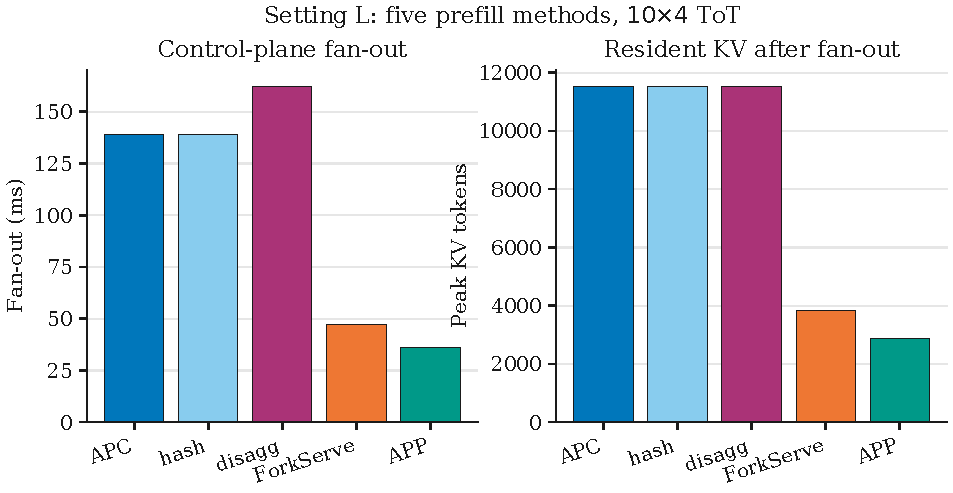
\includegraphics[width=\textwidth]{fig/app_prefill_methods.pdf}
\caption{Setting L visualization.
Hash prefill matches APC on the first expand.
Stock disaggregated prefill is slower because it ships the clone.
ForkServe aliases the trunk; APP also drops the two low-score residuals.}
\end{figure}

Hash prefill matches APC on this first fan-out: the blocks have not been published, so the hash does not remove the clone.
Stock disaggregated prefill pays the same prefill and then ships all $11520$ tokens, which makes fan-out slower ($162$\,ms), consistent with disaggregated prefill not being a throughput feature.
ForkServe removes the clone by aliasing the trunk ($47$\,ms, peak $3840$).
APP also drops the two low-score residuals, so prefill tokens fall to $2912$, fan-out to $35.9$\,ms, and peak KV to the winner spine ($2880$).
Replay of the committed winner is a full hash hit for APC, hash prefill, and APP (zero extra prefill tokens): hash prefill pays off on the next session, not on the first expand.

The decode-token curve in this setting is a stop model, not a second GPU pass.
On a trace whose accuracy is the GSM8K score $0.845$, ending the winner at an answer marker $60\%$ of the way through a $256$-token budget reaches that accuracy at $153$ decode tokens instead of $256$.
Setting M measures that same stop list on A100s.
The concurrency numbers in setting K remain the system-level capacity claim, because they plug measured peaks ($1563$ vs.\ $1163$) into \eqref{eq:conc}.

\section{GPU APP and decoding acceleration (setting M)}

Setting M is the GPU counterpart of settings K and L.
Qwen3-8B, \texttt{bfloat16}, $80$ items per file, batches of eight, decode budget $D{=}512$, Tree-of-Thoughts $k{=}4$ on GSM8K and Game24, ReAct wrap+recovery $k{=}2$ on HumanEval.
Systems: recompute, APC, ForkServe, ForkServe+ (\texttt{plus\_config}: lazy abort, pointer swap, prune, hash skip, disagg gate, \texttt{decode\_stop}).
Tensor parallel $2$ (GPU $0,1$) and $4$ (GPU $0$--$3$) on the same four A100-SXM4 40GB node.
Scores are official extractors on the stored traces: GSM8K accuracy, Game24 success, HumanEval pass@1.
ForkServe+ on HumanEval uses the ReAct path without draft prune (\texttt{prefilled\_branches}${=}0$), so that column is CoW plus whatever stop markers appear in code.

\subsection{GSM8K: decode stop moves wall-clock}

\begin{table}[h]
\centering
\small
\begin{tabular}{@{}lrrrrrrr@{}}
\toprule
$\mathrm{tp}$ & System & e2e (s) & fan-out (ms) & peak KV & decode tok & tok/item & acc. \\
\midrule
$2$ & recompute & $37.34$ & $2006$ & $4744$ & $40960$ & $512$ & $0.925$ \\
$2$ & APC & $36.00$ & $558$ & $1582$ & $40960$ & $512$ & $0.900$ \\
$2$ & ForkServe & $36.04$ & $1181$ & $1182$ & $21235$ & $265$ & $0.887$ \\
$2$ & ForkServe+ & $28.22$ & $1261$ & $1182$ & $13356$ & $167$ & $0.863$ \\
$4$ & recompute & $23.36$ & $1236$ & $4744$ & $40960$ & $512$ & $0.925$ \\
$4$ & APC & $22.72$ & $438$ & $1582$ & $40960$ & $512$ & $0.938$ \\
$4$ & ForkServe & $23.30$ & $994$ & $1182$ & $20997$ & $262$ & $0.925$ \\
$4$ & ForkServe+ & $16.94$ & $1048$ & $1182$ & $12826$ & $160$ & $0.925$ \\
\bottomrule
\end{tabular}
\caption{Setting M, GSM8K prefix $n{=}80$, $D{=}512$.
Peak KV is identical at $\mathrm{tp}{=}2$ and $\mathrm{tp}{=}4$: occupancy tracks the committed spine, not the rank count.
ForkServe+ / APC peak $=1182/1582{=}0.75$.
Decode tokens follow \eqref{eq:dec-stop}: APC always spends $nD$; ForkServe already hits EOS ($0.52\times$); the stop list cuts that to $0.33\times$ and e2e to $0.78\times$ APC at $\mathrm{tp}{=}2$ and $0.75\times$ at $\mathrm{tp}{=}4$.
Accuracy at four GPUs is $74/80$ vs.\ APC $75/80$.}
\end{table}

\begin{figure}[h]
\centering
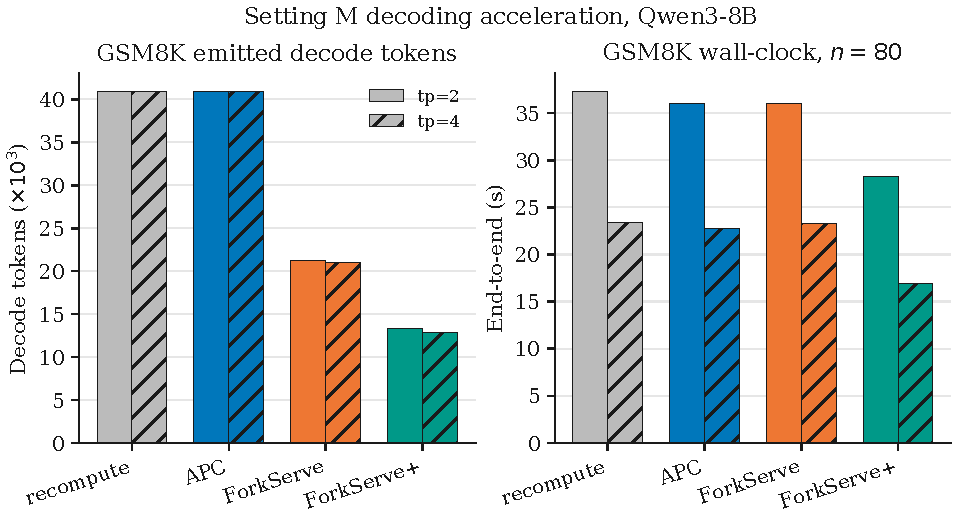
\includegraphics[width=\textwidth]{fig/plus_gsm8k_decode_e2e.pdf}
\caption{Setting M, GSM8K.
Hatched bars are $\mathrm{tp}{=}4$.
APC spends the full $nD$ budget; ForkServe already stops on EOS; ForkServe+ stops at \texttt{\#\#\#\#}.
End-to-end follows $D^{+}$, not fan-out.}
\end{figure}

\begin{figure}[h]
\centering
\begin{minipage}{0.49\textwidth}
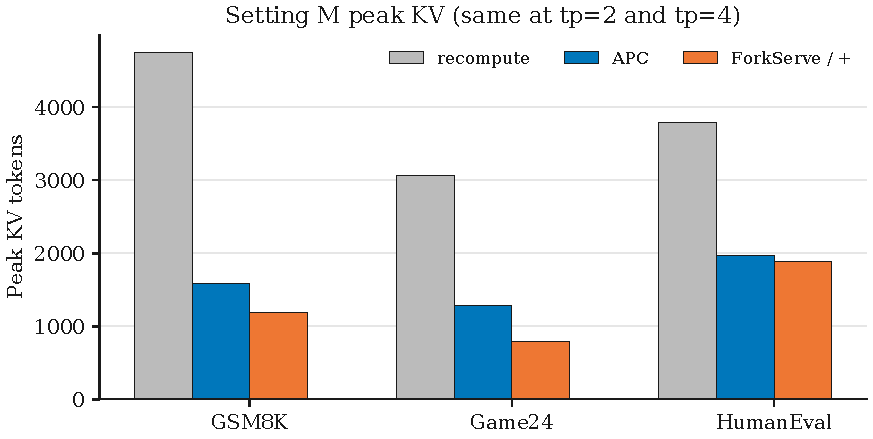
\includegraphics[width=\linewidth]{fig/plus_peak_kv.pdf}
\end{minipage}\hfill
\begin{minipage}{0.49\textwidth}
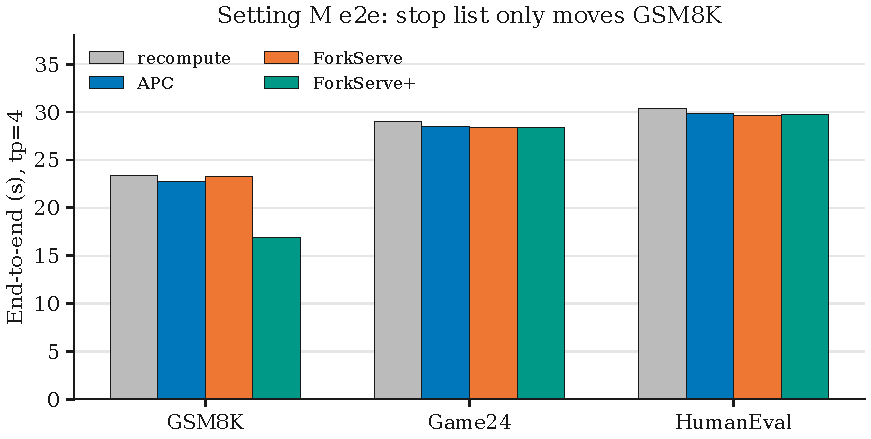
\includegraphics[width=\linewidth]{fig/plus_e2e_tp4.pdf}
\end{minipage}
\caption{Setting M storage vs.\ latency.
Left: peak KV is identical for ForkServe and ForkServe+, below APC on ToT ($0.75\times$, $0.62\times$) and close on ReAct ($0.96\times$).
Right: at $\mathrm{tp}{=}4$, only GSM8K e2e drops, because Game24 and HumanEval do not hit the stop list.}
\end{figure}

$T_{\mathrm{dec}}$ is $26.9$\,s of $28.2$\,s at $\mathrm{tp}{=}2$ for ForkServe+ and $15.9$\,s of $16.9$\,s at $\mathrm{tp}{=}4$.
The e2e gap versus APC is therefore the decode gap, not a faster fan-out: ForkServe+ fan-out is still $1261$\,ms vs.\ APC $558$\,ms at $\mathrm{tp}{=}2$, the same expand overhead the 14B forest showed.
APP's control-plane prune ($p_{\mathrm{d}}{=}1/2$ on synthetic illegal thoughts) does not fire on these GSM8K thoughts---\texttt{pruned\_branches}${=}0$, \texttt{prefilled\_branches}${=}40$ (four thoughts per chunk $\times$ ten chunks)---so the GPU expand path is still CoW of every residual.
What \emph{does} fire is the disagg gate (\texttt{transfer\_tokens}${=}960$ vs.\ a full clone of the live KV) and the stop list.
That is the experimental split: setting L isolates prune on a workload designed to fail the draft score; setting M isolates decode acceleration on a workload that emits \texttt{\#\#\#\#}.

\subsection{Game24 and HumanEval}

\begin{table}[h]
\centering
\small
\resizebox{\textwidth}{!}{%
\begin{tabular}{@{}llrrrrrrr@{}}
\toprule
$\mathrm{tp}$ & System & Game24 e2e (s) & peak & decode tok & success & HE e2e (s) & HE peak & HE pass@1 \\
\midrule
$2$ & recompute & $43.97$ & $3068$ & $40960$ & $0.375$ & $45.90$ & $3796$ & $0.425$ \\
$2$ & APC & $43.14$ & $1289$ & $40960$ & $0.463$ & $44.78$ & $1970$ & $0.438$ \\
$2$ & ForkServe & $42.98$ & $793$ & $35419$ & $0.438$ & $44.64$ & $1882$ & $0.450$ \\
$2$ & ForkServe+ & $43.05$ & $793$ & $34427$ & $0.350$ & $44.70$ & $1882$ & $0.450$ \\
$4$ & recompute & $28.97$ & $3068$ & $40960$ & $0.487$ & $30.42$ & $3796$ & $0.450$ \\
$4$ & APC & $28.51$ & $1289$ & $40960$ & $0.338$ & $29.85$ & $1970$ & $0.425$ \\
$4$ & ForkServe & $28.36$ & $793$ & $35513$ & $0.463$ & $29.69$ & $1882$ & $0.450$ \\
$4$ & ForkServe+ & $28.40$ & $793$ & $34055$ & $0.375$ & $29.77$ & $1882$ & $0.412$ \\
\bottomrule
\end{tabular}%
}
\caption{Setting M, Game24 and HumanEval, $n{=}80$.
Peak ratios vs.\ APC: Game24 $793/1289{=}0.62$, HumanEval $1882/1970{=}0.96$ (wrap-dominated, $k{=}2$), matching \eqref{eq:gap}.
Decode tokens barely move, so e2e stays within $1\%$ of APC.
Game24 success under ForkServe+ is lower than ForkServe at both widths; HumanEval pass@1 is matched at $\mathrm{tp}{=}2$ and $-3$ problems at $\mathrm{tp}{=}4$.}
\end{table}

Game24 traces often fill the $512$-token budget with arithmetic search; HumanEval almost never emits \texttt{\#\#\#\#} or \texttt{\textbackslash boxed}.
\eqref{eq:dec-stop} then predicts $D^{+}\approx nD$ and $T_{\mathrm{e2e}}^{+}\approx T_{\mathrm{e2e}}^{\mathrm{APC}}$, which is what the table shows.
The storage claim still holds: Game24 is the largest abort gap on this node ($0.62\times$ APC), HumanEval the smallest, independent of $\mathrm{tp}$.

\subsection{What setting M adds to L and A}

\begin{itemize}
\item \textbf{Prefill pruning on GPU.} Real GSM8K/Game24 thoughts pass the draft heuristic, so $W_{\mathrm{APP}}\approx W_{\mathrm{FS}}$ on this forest.
The modeled $74\%$ prefill cut in setting L is the illegal-residual case, not the default ToT case.
The GPU still records a disagg transfer of $960$ GSM8K tokens and $1238$ Game24 tokens---survivors only---against a would-be clone of thousands of live tokens under stock disagg.
\item \textbf{Decoding acceleration on GPU.} GSM8K is the positive case of \eqref{eq:dec-stop}: $0.33\times$ decode tokens, $0.75$--$0.78\times$ e2e, accuracy within one problem of APC at $\mathrm{tp}{=}4$.
\item \textbf{KV vs.\ latency.} Peak KV is the same number as ForkServe ($1182$ / $793$ / $1882$) and still below APC at every width.
Efficient serving here is $M_{\mathrm{spine}}$ plus $D^{+}$, not a faster expand.
\end{itemize}

\section{Six-model GPU forest (setting N)}

Setting N is the cross-family check of settings M and \eqref{eq:gap}.
The same four systems, $n{=}40$, batches of eight, $D{=}512$, $\mathrm{tp}{=}2$ and $\mathrm{tp}{=}4$, on Qwen3-4B, Qwen2.5-Math-1.5B, Qwen3-14B, Llama-3-8B-Instruct, Mistral-7B-Instruct-v0.3, and DeepSeek-R1-Distill-Llama-8B.
GSM8K and Game24 run on every model; HumanEval additionally on Llama-3-8B, Mistral-7B, and Qwen3-14B.
Peak KV is identical at both tensor widths on every file.

\subsection{Peak KV holds across families}

\begin{table}[h]
\centering
\small
\resizebox{\textwidth}{!}{%
\begin{tabular}{@{}lrrrrrr@{}}
\toprule
GSM8K, $\mathrm{tp}{=}2$ & Qwen3-4B & Math-1.5B & Qwen3-14B & Llama-3-8B & Mistral-7B & R1-8B \\
\midrule
APC peak & $1512$ & $1512$ & $1512$ & $1509$ & $1569$ & $1405$ \\
FS / FS+ peak & $1112$ & $1112$ & $1112$ & $1109$ & $1169$ & $1005$ \\
ratio vs.\ APC & $0.74$ & $0.74$ & $0.74$ & $0.73$ & $0.75$ & $0.72$ \\
APC $D^{+}$ & $20480$ & $20480$ & $20480$ & $20480$ & $20480$ & $20480$ \\
FS $D^{+}$ & $9860$ & $17070$ & $12087$ & $5560$ & $10013$ & $14974$ \\
FS+ $D^{+}$ & $7206$ & $11704$ & $11162$ & $5262$ & $9660$ & $6422$ \\
APC acc. & $0.925$ & $0.225$ & $0.850$ & $0.625$ & $0.500$ & $0.650$ \\
FS acc. & $0.875$ & $0.275$ & $0.825$ & $0.675$ & $0.475$ & $0.650$ \\
FS+ acc. & $0.550$ & $0.275$ & $0.725$ & $0.675$ & $0.350$ & $0.000$ \\
APC e2e (s) & $14.00$ & $8.31$ & $35.92$ & $11.44$ & $16.14$ & $21.43$ \\
FS e2e (s) & $14.28$ & $8.63$ & $36.20$ & $11.67$ & $18.33$ & $21.74$ \\
FS+ e2e (s) & $12.56$ & $8.63$ & $36.10$ & $11.07$ & $18.10$ & $14.70$ \\
\bottomrule
\end{tabular}%
}
\caption{Setting N, GSM8K $n{=}40$, $\mathrm{tp}{=}2$.
Peak KV is $0.72$--$0.75\times$ APC on every family and does not change at $\mathrm{tp}{=}4$.
ForkServe accuracy stays with APC ($\pm 2$ problems except Math-1.5B, where both are weak).
ForkServe+ stop is safe on Llama-3-8B, cuts tokens on Qwen without always matching accuracy, and zeros DeepSeek-R1 because \texttt{</think>} fires before the answer.}
\end{table}

\begin{figure}[h]
\centering
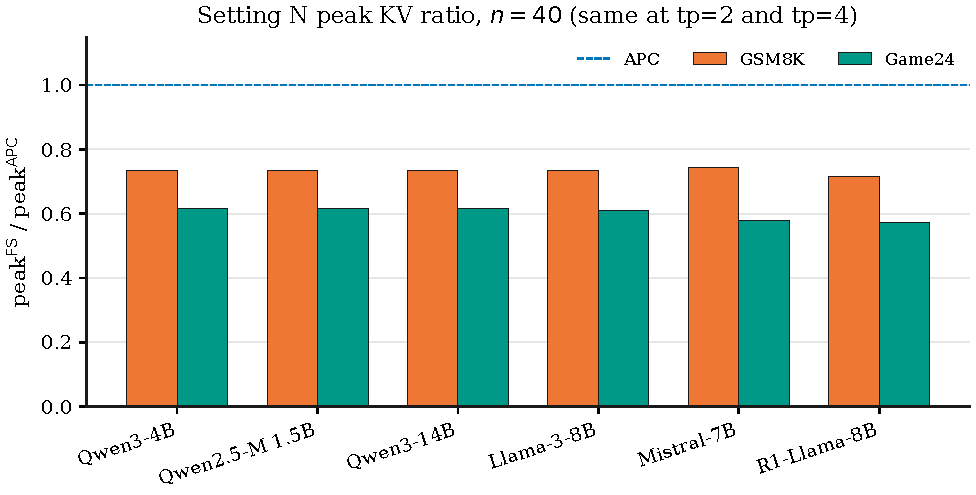
\includegraphics[width=\textwidth]{fig/multi_peak_ratio.pdf}
\caption{Setting N peak-KV ratio vs.\ APC.
GSM8K sits in $[0.72,0.75]$; Game24 in $[0.57,0.62]$.
The abort gap of \eqref{eq:gap} is a property of $k$ and residual length, not of the weight family.}
\end{figure}

\begin{table}[h]
\centering
\small
\begin{tabular}{@{}lrrr@{}}
\toprule
Game24 peak (any $\mathrm{tp}$) & APC & FS / FS+ & ratio \\
\midrule
Qwen3-4B / Math-1.5B / Qwen3-14B & $1287$ & $791$ & $0.61$ \\
Llama-3-8B & $1248$ & $760$ & $0.61$ \\
Mistral-7B & $1351$ & $783$ & $0.58$ \\
DeepSeek-R1-8B & $1144$ & $656$ & $0.57$ \\
\bottomrule
\end{tabular}
\caption{Game24 peak KV.
Short trunks make unused residuals a larger fraction of $M_{\mathrm{APC}}$, so the ratio is below GSM8K, as \eqref{eq:gap} predicts.}
\end{table}

HumanEval wrap+recovery ($k{=}2$) on Llama-3-8B, Mistral-7B, and Qwen3-14B keeps peak $1624/1800{=}0.90$, $1828/2052{=}0.89$, and $1538/1626{=}0.95$ vs.\ APC: the wrap residual is long relative to $L$, so $\Delta$ shrinks.
Official pass@1 on Mistral-7B is $0.350$ ($14/40$) for recompute, APC, ForkServe, and ForkServe+ at both tensor widths; Llama-3-8B and Qwen3-14B stay within two problems of APC.

\begin{table}[h]
\centering
\small
\begin{tabular}{@{}lrrr@{}}
\toprule
HumanEval pass@1, $n{=}40$, $\mathrm{tp}{=}2$ & Llama-3-8B & Mistral-7B & Qwen3-14B \\
\midrule
recompute & $0.550$ & $0.350$ & $0.525$ \\
APC & $0.500$ & $0.350$ & $0.575$ \\
FS / FS+ & $0.475$ & $0.350$ & $0.550$ \\
peak FS / APC & $0.90$ & $0.89$ & $0.95$ \\
APC e2e (s) & $12.75$ & $11.69$ & $37.71$ \\
FS e2e (s) & $14.93$ & $13.77$ & $37.55$ \\
\bottomrule
\end{tabular}
\caption{Setting N HumanEval.
Mistral pass@1 is $0.350$ on every system (same at $\mathrm{tp}{=}4$).
Peak ratios stay wrap-dominated ($k{=}2$).
At $\mathrm{tp}{=}4$, Llama is $0.600$ / $0.600$ / $0.575$ and Qwen3-14B is $0.525$ / $0.575$ / $0.575$ (recompute / APC / FS).}
\end{table}

\subsection{Decode stop is not portable}

\begin{figure}[h]
\centering
\begin{minipage}{0.49\textwidth}
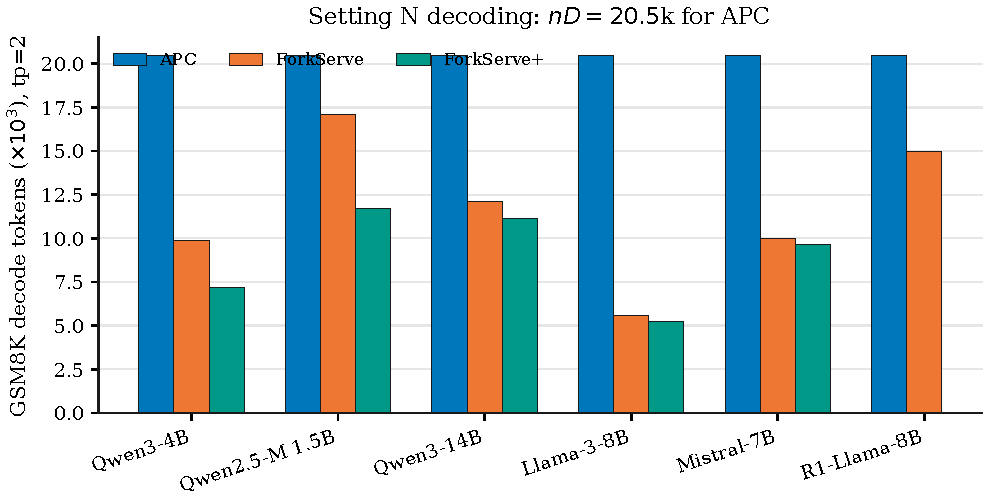
\includegraphics[width=\linewidth]{fig/multi_gsm8k_decode.pdf}
\end{minipage}\hfill
\begin{minipage}{0.49\textwidth}
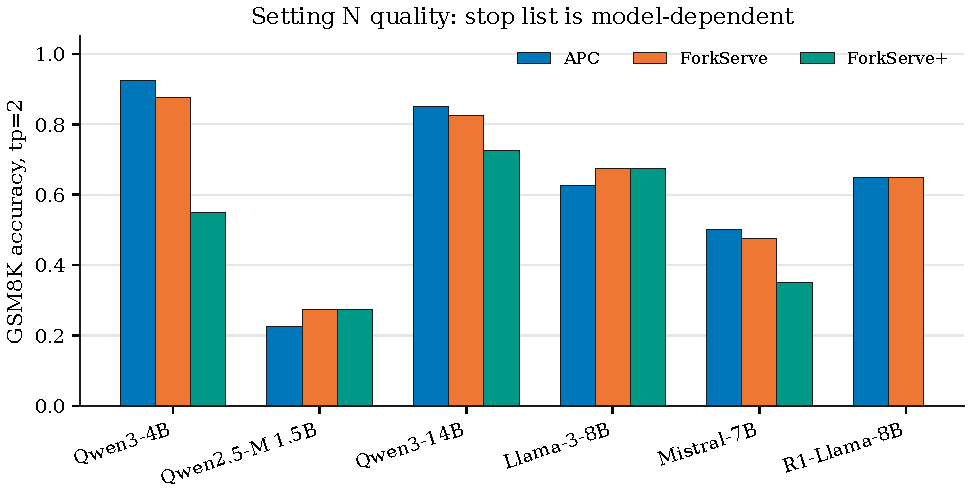
\includegraphics[width=\linewidth]{fig/multi_gsm8k_acc.pdf}
\end{minipage}
\caption{Setting N GSM8K, $\mathrm{tp}{=}2$.
Left: APC always emits $nD$; ForkServe already stops on EOS; ForkServe+ stops earlier.
Right: ForkServe tracks APC accuracy; ForkServe+ matches on Llama-3-8B, drops on Qwen3-4B / Mistral / Qwen3-14B, and fails on DeepSeek-R1 when \texttt{</think>} is a stop string.}
\end{figure}

The storage identity is the transferable result of setting N.
Answer-marker stop transfers only when the model actually writes \texttt{\#\#\#\#} or \texttt{\textbackslash boxed} after a complete answer, as on Qwen3-8B in setting M.
On DeepSeek-R1, \texttt{</think>} is part of the reasoning trace, so FS+ e2e falls ($14.7$\,s vs.\ $21.4$\,s) with accuracy $0$.
On Llama-3-8B, FS+ keeps accuracy $0.675$ at $0.26\times$ APC decode tokens.
Use ForkServe (no stop list) when comparing quality across families; use ForkServe+ only on chat templates that emit a dedicated answer marker.

At $\mathrm{tp}{=}4$, peak KV is unchanged and wall-clock scales by $0.60$--$0.72$ vs.\ $\mathrm{tp}{=}2$ on GSM8K for APC and ForkServe, the same decode-bound scaling as settings E--J.

\section{Discussion}

Recompute copies the trunk on every branch; APC reuses it after a hash hit and already removes most of $M_{\mathrm{rec}}$.
ForkServe is branch-aware KV sharing: it keeps that prefill saving, then drops unused branches so peak KV tracks $M_{\mathrm{spine}}$.
On GSM8K that is $0.72\times$ APC and $0.25\times$ recompute in every batch, while generation time stays within $2\%$ of APC when the decode budget is spent in full.
Fan-out carries copy-on-write and abort; global latency follows $T_{\mathrm{dec}}$ and $C\propto\mathrm{HBM}/M$, so the serving optimum in \eqref{eq:conc} is less HBM than APC at matched $T_{\mathrm{e2e}}$.
APP and answer-marker stop are the two knobs that then cut $T_{\mathrm{fan}}$ and $D$.
Settings B and C check Game24, HumanEval, and $\mathrm{tp}{=}2$ versus $\mathrm{tp}{=}4$; GSM8K quality at full $n$ is setting A.
Settings G and H run the seven-file math suite on Qwen3-14B: the same peak ratios $0.62$--$0.80$, pool accuracy within $7$ problems of APC, and $T_{\mathrm{e2e}}$ within a few percent, with four-GPU wall-clock $0.61$--$0.64\times$ two GPUs.
Settings E and F repeat that recipe on Qwen3-8B, where four-GPU time scales by $0.66$.
Settings I and J repeat it on DeepSeek-R1-Distill-Llama-8B with $D{=}2048$: peak $0.58$--$0.77\times$ APC, pool accuracy $+10$ and $+11$ problems, and four-GPU time $0.56$--$0.64\times$ two GPUs.
Setting K plugs those GSM8K peaks into \eqref{eq:conc}: $35\%$ more concurrent trees, $35\%$ more saturated tok/s, and SLO-feasible QPS $256$ vs.\ $192$.
Setting L places APP against hash prefill and disaggregated prefill on a fan-out with illegal residuals: hash prefill does not help until blocks are published, disaggregated prefill adds a transfer, and APP is the method whose modeled fan-out is below APC.
Setting M runs the same ForkServe+ stack on A100s for Qwen3-8B: KV still $0.62$--$0.75\times$ APC on ToT, GSM8K decode tokens $0.33\times$ APC, GSM8K e2e $0.75$--$0.78\times$ APC, and Game24/HumanEval e2e matched because those traces do not hit the stop list.
Setting N repeats the forest on six models ($n{=}40$): GSM8K peak $0.72$--$0.75\times$ APC and Game24 $0.57$--$0.62\times$ on every family; ForkServe accuracy tracks APC; ForkServe+ stop is not portable (DeepSeek-R1 accuracy $0$ when \texttt{</think>} is a stop string).
HumanEval pass@1 on Mistral-7B is $0.350$ for every system, with peak $0.89\times$ APC.

\section{Conclusion}

ForkServe is efficient vLLM serving of Tree-of-Thoughts and ReAct: the trunk is forked by copy-on-write, unused branches are aborted, residuals can be pruned before prefill, and winner decode can stop at an answer marker.
Against recompute, the relevant quantities are prefill work
$W_{\mathrm{rec}}=k(L+\bar\ell)$ versus $W_{\mathrm{FS}}=L+k\bar\ell$,
and clone memory $M_{\mathrm{rec}}$ versus the committed path $M_{\mathrm{spine}}=b(L+\ell_{\star})$.
Against APC, prefill matches until APP drops losers \eqref{eq:app-w}, and the remaining storage gap is
\begin{equation}
\Delta = M_{\mathrm{APC}}-M_{\mathrm{spine}} = b\sum_{i\neq\star}\ell_i,
\end{equation}
the hashed union that remains under APC.
A run is efficient when \eqref{eq:goal} holds, official scores stay with APC, and---when a stop marker exists---$D^{+}<nD$ as in \eqref{eq:dec-stop}.
The serving objective is system throughput $\Theta\propto C/T_{\mathrm{e2e}}$ with $C\propto\mathrm{HBM}/M$ (\eqref{eq:conc}).

The completed measurements support that claim on more than one task, tensor-parallel width, and model size.
The GSM8K test set ($n{=}1319$, $\mathrm{tp}{=}2$, Qwen3-14B) is the main Tree-of-Thoughts result: peak KV below APC on all $165$ batches (median ratio $0.72$), accuracy aligned with APC, and $T_{\mathrm{e2e}}$ within $2\%$ without decode-stop.
Four-problem slices reproduce the same storage ordering on Tree-of-Thoughts (GSM8K, Game24) and ReAct (HumanEval) at $\mathrm{tp}{=}2$, and on Game24 and HumanEval at $\mathrm{tp}{=}4$.
On Qwen3-14B (settings G and H) and Qwen3-8B (settings E and F), seven math files give $\mathrm{peak}^{\mathrm{FS}}/\mathrm{peak}^{\mathrm{APC}}\in[0.62,0.80]$ at both $\mathrm{tp}{=}2$ and $\mathrm{tp}{=}4$.
On DeepSeek-R1-Distill-Llama-8B (settings I and J) the same files with $D{=}2048$ give $\mathrm{peak}^{\mathrm{FS}}/\mathrm{peak}^{\mathrm{APC}}\in[0.58,0.77]$, micro-accuracy $+2.0$ and $+2.1$\,pp over APC, and $T_{\mathrm{e2e}}$ $-0.5\%$ / $+1.3\%$.
Generate time at four GPUs is $0.56$--$0.66\times$ the two-GPU run and stays with APC.
Where $k{=}4$, $M_{\mathrm{spine}}/M_{\mathrm{APC}}$ sits in $[0.58,0.80]$; where $k{=}2$, the ratio rises to $0.94$, as \eqref{eq:gap} predicts when residuals are large relative to $L$.
Setting K turns that $M$ gap into concurrency: $C^{\mathrm{FS}}/C^{\mathrm{APC}}{=}50/37$ and $35\%$ more peak tok/s under a $1\,\mathrm{s}$ P99 TTFT SLO.

Setting L is the design response to the fan-out term that still limits $\Theta$.
$T_{\mathrm{fan}}^{\mathrm{FS}}$ is above $T_{\mathrm{fan}}^{\mathrm{APC}}$ on the GPU forest; APP moves hash skip, draft prune, early abort, and the disagg \texttt{insert} gate in front of that expand.
The control-plane ordering is APP, then ForkServe, then APC / hash prefill, then stock disaggregated prefill.
Setting M confirms two GPU facts on Qwen3-8B ($n{=}80$).
First, real ToT thoughts do not trip the draft heuristic, so expand is still CoW of every residual and still slower than APC.
Second, GSM8K answer-marker stop is a real latency win: $0.33\times$ decode tokens and $0.75\times$ e2e at $\mathrm{tp}{=}4$ with accuracy $0.925$ vs.\ $0.938$.
Game24 and HumanEval keep APC-level e2e because those traces do not hit the stop list, while peak KV remains below APC ($0.62\times$ and $0.96\times$).
Setting N extends that storage claim to six families at $n{=}40$: GSM8K peak $0.72$--$0.75\times$ APC, Game24 $0.57$--$0.62\times$, ForkServe accuracy with APC, and ForkServe+ stop not portable (DeepSeek-R1 accuracy $0$).
Mistral-7B HumanEval pass@1 is $0.350$ ($14/40$) on recompute, APC, and ForkServe.

The remaining full-set runs are Tree-of-Thoughts on Game24 ($n{=}1362$) and ReAct on HumanEval ($n{=}164$) for ForkServe; vLLM recompute and APC already finished those files.
A live-scheduler concurrent-load experiment should likewise confirm the analytical $C$ and $\Theta$ of setting K.

\end{document}
